\documentclass[12pt,a4paper]{article}
%
%	STARWARE - Stile base per la scrittura di documenti interni in LaTex
%

%
%	Pacchetti globali
%	Fare qui eventuali aggiunte!
%
\usepackage[utf8]{inputenc}
\usepackage[italian]{babel}
\usepackage[babel]{csquotes}
\usepackage{url}
\usepackage{graphicx}
\usepackage[colorlinks]{hyperref}
\usepackage{lastpage}
\usepackage{fancyhdr}
\usepackage[top=1cm,bottom=4cm,left=80pt,right=80pt]{geometry} %disegna la linea
\usepackage{listings} %per grandi porzioni di codice
\usepackage{color}
\usepackage[table]{xcolor}
\usepackage{booktabs,tabularx}
\usepackage{makeidx}
\usepackage{fixltx2e}
\usepackage{hyperref}
\usepackage{enumitem}
\usepackage{color}
\usepackage[T1]{fontenc}
\usepackage{float}
\usepackage{svg}
\usepackage{amsmath}
\usepackage[toc]{glossaries}
\usepackage{dirtree}
\usepackage{listings}

\makeglossaries

\bibliographystyle{alpha}

%
%	VARIABILI GLOBALI
%
\newcommand{\nomeGruppo}{StarWare}
\newcommand{\mailGruppo}{starware.swe@gmail.com}
\newcommand{\uni}{Universit\`{a} degli Studi di Padova}
\newcommand{\uniAA}{2015/2016}
\newcommand{\Cardin}{Prof. Riccardo Cardin}
\newcommand{\Vardanega}{Prof. Tullio Vardanega}
\newcommand{\Zucchetti}{Zucchetti S.p.a.}
\newcommand{\prj}{Quizzipedia}
\newcommand{\prjL}{Quizzipedia: software per la gestione di questionari}

\newcommand{\AVI}{Alessio Vitella}
\newcommand{\AVE}{Andrea Venier}
\newcommand{\NDC}{Nicola De Cao}
\newcommand{\IB}{Igor Baylyak}
\newcommand{\WS}{Walter Sandon}
\newcommand{\TP}{Thomas Pigarelli}
\newcommand{\AB}{Anna Bonaldo}

\newcommand{\mgls}[1]{\gls{#1}\textsubscript{G}}
\newcommand{\mglspl}[1]{\glspl{#1}\textsubscript{G}}
\newcommand{\mGls}[1]{\Gls{#1}\textsubscript{G}}
\newcommand{\mGlspl}[1]{\Glspl{#1}\textsubscript{G}}

\newcommand{\AM}{\emph{\mGls{amministratore}}}
\newcommand{\AN}{\emph{\mGls{analista}}}
\newcommand{\PG}{\emph{\mGls{progettista}}}
\newcommand{\PR}{\emph{\mGls{programmatore}}}
\newcommand{\VR}{\emph{\mGls{verificatore}}}
\newcommand{\PM}{\emph{\mGls{project manager}}}

\newcommand{\AMpl}{\emph{\mGlspl{amministratore}}}
\newcommand{\ANpl}{\emph{\mGlspl{analista}}}
\newcommand{\PGpl}{\emph{\mGlspl{progettista}}}
\newcommand{\PRpl}{\emph{\mGlspl{programmatore}}}
\newcommand{\VRpl}{\emph{\mGlspl{verificatore}}}
\newcommand{\PMpl}{\emph{\mGlspl{project manager}}}

\newcommand{\RR}{\emph{\mGls{revisione dei requisiti}}}
\newcommand{\RA}{\emph{\mGls{revisione di accettazione}}}
\newcommand{\RP}{\emph{\mGls{revisione di progettazione}}}
\newcommand{\RQ}{\emph{\mGls{revisione di qualifica}}}

\newcommand{\NdP}{\emph{\mGls{norme di progetto}}}
\newcommand{\SdF}{\emph{\mGls{stidio di fattibilita}}}
\newcommand{\AdR}{\emph{\mGls{analisi dei requisiti}}}
\newcommand{\PdP}{\emph{\mGls{piano di progetto}}}
\newcommand{\PdQ}{\emph{\mGls{piano di qualifica}}}

\newcommand{\latex}[1]{\texttt{#1}}
\newcommand{\fileName}[1]{\texttt{#1}}
\newcommand{\filePath}[1]{\texttt{#1}}
\newcommand{\TODO}[1]{\texttt{\large \color{red} \underline{TODO: #1}}}

\newcommand{\licenza}{GNU GENERAL PUBLIC LICENSE V2}

%per compilare il template usare questi sotto e commentare glia altri:
%\newcommand{\logoLungo}{../imgs/logoLungo.png}
%\newcommand{\logoGrande}{../imgs/logoGrande.png}
\newcommand{\logoLungo}{../../../template/imgs/logoLungo.png}
\newcommand{\logoGrande}{../../../template/imgs/logoGrande.png}

%
%	Setup stili
%

\newcommand{\HRule}{\rule{\linewidth}{0.5mm}}

\definecolor{dkgreen}{rgb}{0,0.6,0}
\definecolor{gray}{rgb}{0.5,0.5,0.5}
\definecolor{mauve}{rgb}{0.58,0,0.82}
\definecolor{light}{RGB}{255,255,190}

%
%	Setup di pagina
%

%colorazione link
\hypersetup
{
	colorlinks=true,
	linkcolor=black,
	urlcolor=blue,
	citecolor=blue
}

%	Setup Header + Footer

\pagestyle{fancy}
\setlength{\headheight}{2cm} %settato grandezza header

\renewcommand{\footrulewidth}{0.5pt} %ridefinisco il valore della riga di intestazione
\renewcommand{\headrulewidth}{0.5pt} %ridefinisco il valore della riga di pie' di pagina
\addtolength{\headwidth}{\marginparsep}
\addtolength{\headwidth}{\marginparwidth}

\fancyhead{} %annulla head di default
\fancyfoot{} %annulla foot di default

%	Logo intestazione
\lhead{
\includegraphics[scale=0.12]{\logoLungo}}


%	footer
\cfoot{
	\uni \ - \uniAA \\
	\href{mailto:\mailGruppo}{\mailGruppo}\\
	{\tiny Questo documento è distribuito sotto licenza {\licenza}}
}
\rfoot{
	\thepage\ di \pageref{LastPage}
}


% test subsubsubsection

\usepackage{titlesec}
\usepackage{hyperref}

\titleclass{\subsubsubsection}{straight}[\subsection]

\newcounter{subsubsubsection}[subsubsection]
\renewcommand\thesubsubsubsection{\thesubsubsection.\arabic{subsubsubsection}}
\renewcommand\theparagraph{\thesubsubsubsection.\arabic{paragraph}} % optional; useful if paragraphs are to be numbered

\titleformat{\subsubsubsection}
  {\normalfont\normalsize\bfseries}{\thesubsubsubsection}{1em}{}
\titlespacing*{\subsubsubsection}
{0pt}{3.25ex plus 1ex minus .2ex}{1.5ex plus .2ex}

\makeatletter
\renewcommand\paragraph{\@startsection{paragraph}{5}{\z@}%
  {3.25ex \@plus1ex \@minus.2ex}%
  {-1em}%
  {\normalfont\normalsize\bfseries}}
\renewcommand\subparagraph{\@startsection{subparagraph}{6}{\parindent}%
  {3.25ex \@plus1ex \@minus .2ex}%
  {-1em}%
  {\normalfont\normalsize\bfseries}}
\def\toclevel@subsubsubsection{4}
\def\toclevel@paragraph{5}
\def\toclevel@paragraph{6}
\def\l@subsubsubsection{\@dottedtocline{4}{7em}{4em}}
\def\l@paragraph{\@dottedtocline{5}{10em}{5em}}
\def\l@subparagraph{\@dottedtocline{6}{14em}{6em}}
\makeatother

\setcounter{secnumdepth}{4}
\setcounter{tocdepth}{4}


%pdflatex -synctex=1 -interaction=nonstopmode %.tex|makeglossaries %|pdflatex -synctex=1 -interaction=nonstopmode %.tex|pdflatex -synctex=1 -interaction=nonstopmode %.tex
\makeglossary

\newglossaryentry{responsabile} {
	name=responsabile,
	description={è il responsabile della gestione, pianificazione e realizzazione del progetto},
	plural=Responsabili
}

\newglossaryentry{verificatore} {
	name=verificatore,
	description={è il responsabile dell'attività di verifica},
	plural=Verificatori
}

\newglossaryentry{programmatore} {
	name=programmatore,
	description={è responsabile delle attività di codifica miranti alla realizzazione del prodotto e delle componenti di ausilio necessarie per l'esecuzione delle prove di verifica e validazione},
	plural=programmatori
}

\newglossaryentry{progettista} {
	name=progettista,
	description={è responsabile delle attività di progettazione},
	plural=Progettisti
}

\newglossaryentry{analista} {
	name=analista,
	description={è responsabile delle attività di analisi. },
	plural=Analisti
}

\newglossaryentry{amministratore} {
	name=amministratore,
	description={è responsabile dell'efficienza e dell'operatività dell'ambiente di sviluppo; si occupa della redazione e attuazione di piani e procedure di gestione della qualità; inoltre gestisce l'archivio della documentazione del progetto},
	plural=Amministratori
}

\newglossaryentry{revisione dei requisiti} {
	name=revisione dei requisiti,
	description={è una revisione formale che determina l'accesso del gruppo al progetto didattico e la concordanza con il cliente di una visione condivisa del prodotto atteso}
}

\newglossaryentry{revisione di accettazione} {
	name=revisione di accettazione,
	description={è una revisione formale per l'accertamento del soddisfacimento di tutti i requisiti e il completamento del progetto}
}

\newglossaryentry{revisione di progettazione} {
	name=revisione di progettazione,
	description={è una revisione di progresso che accerta la realizzabilità del prodotto e informa il cliente sulle caratteristiche del prodotto}
}

\newglossaryentry{revisione di qualifica} {
	name=revisione di qualifica,
	description={è una revisione di progresso che approva l'esito finale delle verifiche e attiva la fase di validazione}
}

\newglossaryentry{analisi} {
	name=analisi,
	description={è il periodo di preparazione e produzioni di documenti che precede la Revisione dei requisiti}
}

\newglossaryentry{progettazione} {
	name=progettazione,
	description={è il periodo che intercorre tra la Revisione dei requisiti e la Revisione di progettazione}
}

\newglossaryentry{codifica} {
	name=codifica,
	description={è il periodo che intercorre tra la Revisione di progettazione e la Revisione di qualifica}
}

\newglossaryentry{validazione} {
	name=validazione,
	description={è il periodo che intercorre tra la Revisione di qualifica e la Revisione di accettazione}
}

\newglossaryentry{repository} {
	name=repository,
	description={è dove i file sono memorizzati, spesso su un server}
}

\newglossaryentry{ruolo} {
	name=ruolo,
	description={una delle figure professionali che una persona fisica interpreta nel corso del progetto. I ruoli sono: responsabile, amministratore, analista, progettista, programmatore e verificatore},
    plural=ruoli
}

\newglossaryentry{svg} {
	name=SVG,
	description={è un formato per la visualizzazione di oggetti in grafica vettoriale. Per maggiori informazioni si veda \href{https://it.wikipedia.org/wiki/Scalable_Vector_Graphics}{qui}}
}

\newglossaryentry{png} {
	name=PNG,
	description={abbreviazione di Portable Network Graphics, è un formato di file per memorizzare immagini. Per ulteriori informazioni si veda \href{http://it.wikipedia.org/wiki/Portable_Network_Graphics}{qui}}
}

\newglossaryentry{pdf} {
	name=PDF,
	description={è un formato di file basato su un linguaggio di descrizione di pagina sviluppato da Adobe Systems nel 1993 per rappresentare documenti in modo indipendente dall’hardware e dal software utilizzati per generarli o per visualizzarli. Per ulteriori informazioni si veda \href{http://it.wikipedia.org/wiki/Portable_Document_Format}{qui}}
}

\newglossaryentry{uml} {
	name=UML,
	description={è un linguaggio di modellazione e specifica basato sul paradigma object-oriented. Per ulteriori informazioni si veda \href{http://it.wikipedia.org/wiki/Unified_Modeling_Language}{qui}}
}

\newglossaryentry{walkthrough} {
	name=walkthrough,
    description={consiste nella lettura di un documento o codice cercando errori ed anomalie senza un'idea precisa di quali tipi di errori sarà possibile trovare}
}

\newglossaryentry{lista di controllo} {
	name=lista di controllo,
	description={è un elenco di cose da fare per eseguire una determinata attività}
}

\newglossaryentry{inspection} {
	name=inspection,
	description={è la lettura mirata di un documento o codice cercando errori specifici}
}

\newglossaryentry{milestone} {
	name=milestone,
	description={momento saliente nello sviluppo di un prodotto software per la quale devono essere pronti documenti e/o funzionalità}
}

\newglossaryentry{ticket} {
	name=ticket,
	description={rappresenta un compito nell'organizzazione e distribuzione del lavoro all'interno del progetto},
	plural=tickets
}

\newglossaryentry{commit} {
	name=commit,
	description={è la copia di modifiche fatte su file locali verso la repository remota. Esso rappresenta anche un particolare stato della repository nel tempo}
}

\newglossaryentry{versionamento} {
	name=versionamento,
	description={è la gestione di un versioni multiple di un insieme di informazioni. Per maggiori informazioni si veda \href{http://it. wikipedia.org/wiki/Controllo_versione}{qui}}
}

\newglossaryentry{task} {
	name=task,
	description={è un compito secondo la definizione dello standard IEEE 12207},
	plural=tasks
}

\newglossaryentry{attivita} {
	name=attivita,
	description={è un insieme di task}
}

\newglossaryentry{redattore} {
	name=redattore,
	description={colui che redige un documento},
	plural=redattori
}

\newglossaryentry{proponente} {
	name=proponente,
	description={colui che ha proposto al committente un capitolato d'appalto}
}

\newglossaryentry{committente} {
	name=committente,
	description={colui che assegna un compito. In questo caso è il Professor Tullio Vardanega}
}

\newglossaryentry{quality assurance} {
	name=quality assurance,
	description={è l'insieme delle attività volte a garantire il soddisfacimento degli obiettivi della qualità}
}

\newglossaryentry{telegram} {
	name=telegram,
	description={è un servizio di messaggistica istantanea utilizzato dal gruppo per comunicazioni interne. Per maggiori informazioni si veda \href{https://it.wikipedia.org/wiki/Telegram_(software)}{qui}}
}

\newglossaryentry{browser} {
	name=browser,
	description={è un'applicazione per il recupero, la presentazione e la navigazione di risorse web}
}

\newglossaryentry{google drive} {
	name=Google Drive,
	description={è un servizio di memorizzazione e sincronizzazione online introdotto da Google il 24 aprile 2012. Per maggiori informazioni si veda \href{https://it.wikipedia.org/wiki/Google_Drive}{qui}}
}

\newglossaryentry{skype} {
	name=Skype,
	description={è un software proprietario freeware di messaggistica istantanea e VoIP. Per maggiori informazioni si veda \href{https://it.wikipedia.org/wiki/Skype}{qui}}
}

\newglossaryentry{gantt} {
	name=Gantt,
	description={è un diagramma di supporto alla gestione dei progetti}
}

\newglossaryentry{projectlibre} {
	name=ProjectLibre,
	description={è un software di gestione progettuale}
}

\newglossaryentry{pert} {
	name=PERT,
	description={è uno strumento volto alla programmazione delle attività che compongono il progetto e, più in generale, alla gestione degli aspetti temporali di quest'ultimo}
}

\newglossaryentry{subtask} {
	name=subtask,
	description={è un task compreso all'interno di un altro task. La totalità di tutti i subtasks costituisce un intero task}
	plural=subtasks
}

\newglossaryentry{ticketing} {
	name=ticketing,
	description={procedura con la quale il Responsabile assegna un task}
}

\newglossaryentry{git} {
	name=git,
	description={è un sistema software di controllo di versione distribuito}
}

\newglossaryentry{quizzpedia} {
	name=Quizzpedia,
	description={è il nome del prodotto software richiesto dal capitolato d'appalto scelto}
}

\newglossaryentry{schierabile} {
	name=schierabile,
	description={è la capacità di rilasciare al cliente, con relativa installazione e messa in funzione o esercizio, di una applicazione o di un sistema software tipicamente all'interno di un sistema informatico aziendale}
}

\newglossaryentry{cross-platform} {
	name=cross-platform,
	description={può essere riferito ad un linguaggio di programmazione, ad un'applicazione software o ad un dispositivo hardware che funziona su più di un sistema}
}

\newglossaryentry{qml} {
	name=QML,
	description={è un "Domain Specific Language" richiesto dal capitolato d'appalto per la definizione delle domande all'interno del sistema}
}

\newglossaryentry{tomcat} {
	name=Tomcat,
	description={è un application server nella forma di contenitore servlet open source sviluppato dalla Apache Software Foundation. Per maggiori informazioni si veda \href{https://it.wikipedia.org/wiki/Apache_Tomcat}{qui}}
}

\newglossaryentry{java} {
	name=Java,
	description={è un linguaggio di programmazione orientato agli oggetti, specificatamente progettato per essere il più possibile indipendente dalla piattaforma di esecuzione. Per maggiori informazioni si veda \href{https://it.wikipedia.org/wiki/Java_(linguaggio_di_programmazione)}{qui}}
}

\newglossaryentry{node.js} {
	name=Node.js,
	description={è un framework che permette di realizzare web application usando un linguaggio di programmazione che utilizza la stessa sintassi di JavaScrip. Utilizza un modello event-driven, anzichè il classico modello a processi o thread concorrenti, e ciò significa che si eseguono azioni solo al verificarsi di un evento. Questo modello asincrono rende leggero ed efficiente, ideale per applicazioni real-time in per dispositivi distribuiti}
}

\newglossaryentry{javascript} {
	name=JavaScript,
	description={linguaggio di scripting orientato agli oggetti comunemente usato nella programmazione
Web}
}

\newglossaryentry{postgresql} {
	name=PostgreSQL,
	description={e un sistema di gestione di basi di dati open source usato per applicazioni che richiedono caratteristiche molto complesse complesse}
}

\newglossaryentry{mongodb} {
	name=MongoDB,
	description={è un sistema gestionale di basi di dati NoSQL orientato ai documenti, adatto per ambienti che hanno la necessità d'immagazzinare grosse quantità di dati, e dove il linguaggio utilizzato per la gestione dei dati è \mgls{javascript}}
}

\newglossaryentry{html5} {
	name=HTML5,
	description={linguaggio di markup per la strutturazione delle pagine web}
}

\newglossaryentry{css3} {
	name=CSS3,
	description={è un linguaggio di programmazione web utilizzato per descrivere l'aspetto e la formattazione di un sito web al browser lato client. }
}

\newglossaryentry{xml} {
	name=XML,
	description={è un meta-linguaggio che fornisce un insieme standard di regole sintattiche per modellare la struttura di documenti e dati. Questo insieme di regole, definiscono le modalità secondo cui è possibile crearsi un proprio linguaggio di markup}
}

\newglossaryentry{nosql} {
	name=NoSQL,
	description={come dice anche il termine questi database non sono basati su SQL, non sono basati su uno schema relazionale. I database relazionali sono infatti ottimi quando esistono delle relazioni tra i dati che salviamo, ma sono poco performanti nel caso sia necessario salvare una grande quantità di dati, magari usando la scalabilità orizzontale, quando cioè si utilizzano più server dove salvare questi dati e non solamente incrementando la potenza di un singolo server.
}
}

\newglossaryentry{scala} {
	name=Scala,
	description={è un linguaggio di programmazione di tipo general-purpose multi-paradigma studiato per integrare le caratteristiche e funzionalità dei linguaggi orientati agli oggetti e dei linguaggi funzionali. Per maggiori informazioni si veda \href{https://it.wikipedia.org/wiki/Scala_(linguaggio_di_programmazione)}{qui}}
}

\newglossaryentry{akka} {
	name=Akka,
	description={è un toolkit di strumenti per la costruzione di applicazioni con elevata concorrenza di dati che necessitano di un sistema resilente per l'invio e la ricezione di messaggi}
}

\newglossaryentry{ble} {
	name=BLE,
	description={Bluetooth low energy,  pur mantenendo un range di comunicazione simile a quello classico, fornisce un  consumo energetico dei device notevolmente ridotto}
}

\newglossaryentry{mqtt} {
	name=MQTT,
	description={è un protocollo di messaggistica leggero posizionato in cima a TCP/IP, disegnato per le situazioni in cui è richiesto un basso impatto e dove la banda è limitata. }
}

\newglossaryentry{aws} {
	name=AWS,
	description={è un insieme di servizi di elaborazione rermoti, detti anche servizi web, che costituiscono una piattaforma di cloud computing offerto da Amazon. Per maggiori informazioni si veda \href{https://aws.amazon.com/it/}{qui}}
}

\newglossaryentry{heroku} {
	name=Heroku,
	description={è una  delle prime cloud Platform-as-a-Service (PaaS) che supportava solo Java come linguaggio di programmazione, oggi giorno ha aggiunto molti altri linguaggi come Scala, Phyton, etc. Per maggiori informazioni si veda \href{https://www.heroku.com}{qui}}
}

\newglossaryentry{github} {
	name=Github,
	description={software di controllo di versione che permette di aggiornare un file senza dover sovrascrivere le versioni precedenti}
}

\newglossaryentry{template} {
	name=template,
	description={traducibile in italiano come modello, indica o un programma o un documento idealizzato come un documento semicompilato cartaceo che ha degli spazi bianchi che saranno successivamente riempiti}
	plural=templates
}

\newglossaryentry{dropbox} {
	name=Dropbox,
	description={è un software di cloud storage multipiattaforma, che offre un servizio di file hosting e sincronizzazione automatica di file tramite web}
}

\newglossaryentry{open-source} {
	name=open-source,
	description={un software di cui gli autori ovvero i detentori dei diritti rendono pubblico il codice sorgente, favorendone il libero studio e permettendo a programmatori indipendenti di apportarvi modifiche ed estensioni. Questo è realizzato tramite apposite licenze d'uso}
}

\newglossaryentry{project management} {
	name=project management,
	description={si intende l'insieme di attività aziendali, svolte tipicamene da una figura dedicata e specializzata detta project manager, volte all'analisi, progettazione, pianificazione e realizzazione degli obiettivi di un progetto, gestendolo in tutte le sue caratteristiche e fasi evolutive, nel rispetto di precisi vincoli come i tempi, costi, risorse, scopi, qualità}
}

\newglossaryentry{linux} {
	name=Linux,
	description={è una famiglia di sistemi operativi open-source di tipo Unix-like, rilasciati sotto varie possibili distribuzioni, aventi la caratteristica comune di utilizzare come nucleo il kernel Linux}
}

\newglossaryentry{windows} {
	name=Windows,
	description={è una famiglia di ambienti operativi e sistemi operativi dedicati ai personal computer, alle workstation, ai server e agli smartphone. Il sistema operativo si chiama così per via della sua interfaccia di programmazione di un'applicazione a finestre}
}

\newglossaryentry{mac os} {
	name=Mac OS,
	description={il sistema operativo di Apple dedicato dedicati ai personal computer Macintosh, alle workstation, ai server e agli smartphone  }
}


\newglossaryentry{schedule variance} {
	name=schedule variance,
	description={ogni deviazione alle baseline di un progetto, misurata confrontando costo preventivato di programma di lavoro con il costo preventivato del lavoro svolto. Indica quindi al cliente se il progetto sta procedendo nei tempi stabiliti}
}

\newglossaryentry{cost variance} {
	name=cost variance,
	description={indica al management aziendale se il valore del costo realmente maturato è maggiore, uguale o minore rispetto al costo pianificato}
}


\newglossaryentry{merge} {
	name=merge,
	description={unire due o più quantità}
}

\newglossaryentry{slack} {
	name=slack,
	description={intervallo di tempo entro cui un evento deve avvenire nel rispetto dei vincoli logici e imposti dal reticolo di pianificazione senza compromettere la durata complessiva del progetto}
}

\newglossaryentry{baseline} {
	name=baseline,
	description={di progetto costituisce il punto di riferimento rispetto al quale calcolare gli scostamenti delle principali variabili implicate nella gestione di un progetto}
}

\newglossaryentry{asana} {
	name=Asana,
	description={è un software che permette a dei team di monitorare il loro lavoro e tener traccia dei risultati tramite l'assegnazione di task a componemti specifiche del gruppo di lavoro}
}

\newglossaryentry{deadline} {
	name=deadline,
	description={La deadline di un \mgls{task} è un indicazione dell'urgenza del \mgls{task}; rappresenta un un punto su una linea temporale ideale. Data di scadenza o termine entro il quale deve essere completato un compito assegnato.}
}

\newglossaryentry{revert} {
	name=revert,
	description={per annullare le ultime modifiche effettuate al repository remoto. Per maggiori informazioni si veda \href{https://git-scm.com/docs/}{qui}}
}

\newglossaryentry{backup} {
	name=backup,
	description={si indica la replicazione, su un qualunque supporto di memorizzazione, di materiale informativo archiviato nella memoria di massa, al fine di prevenire la perdita definitiva dei dati in caso di eventi malevoli accidentali o intenzionali}
}

\newglossaryentry{push} {
	name=push,
	description={per inviare modifiche di un documento site in un host locale al repository remoto. Per maggiori informazioni si veda \href{https://git-scm.com/docs/}{qui}}
}

\newglossaryentry{teamwork} {
	name=teamwork,
	description={è un software che permette a dei team di monitorare il loro lavoro e tener traccia dei risultati tramite l'assegnazione di task a componenti specifiche del gruppo di lavoro}
}

\newglossaryentry{evento} {
	name=evento,
	description={\mgls{teamwork}, attraverso il suo calendario, offre la possibilità di impostare eventi in giorni stabiliti dagli utenti. Questi eventi verranno periodicamente segnalati come promemoria a tutte le persone invitate agli stessi.}
}

\newglossaryentry{etichetta} {
	name=etichetta,
	description={è un controllo grafico che mostra informazioni testuali all'interno di un form}
	plural=etichette
}

\newglossaryentry{bug} {
	name=bug,
	description={identifica un errore nella scrittura di un programma software che ne causa un comportamento imprevisto o comunque diverso da quello specificato dal produttore}
	plural=bugs
}

\newglossaryentry{software} {
	name=software,
	description={e’ un termine generico che definisce programmi e procedure utilizzati per far eseguire al computer un determinato compito}
}

\newglossaryentry{desktop} {
	name=desktop,
	description={area dello schermo su cui appaiono le icone e le finestre rappresentanti le memorie di massa collegate al computer ed il loro contenuto}
}

\newglossaryentry{draw.io} {
	name=draw.io,
	description={é un software gratuito per la creazione di diagrammi di flusso, di processo, UML, e diagrammi di rete}
}

\newglossaryentry{tracy} {
	name=tracy,
	description={software opensource per il tracciamento}
}

\newglossaryentry{package} {
	name=package,
	description={è un meccanismo per organizzare classi Java in gruppi logici, principalmente allo scopo di definire namespace distinti per diversi contesti}
}

\newglossaryentry{stakeholder} {
	name=stakeholder,
	description={si indica genericamente un soggetto o un gruppo di soggetti influenti nei confronti di un'iniziativa economica, sia essa un'azienda o un progetto}
}

\newglossaryentry{branch} {
	name=branch,
	description={quando si vuole creare un nuovo ramo al repository remoto. Per maggiori informazioni si veda \href{https://git-scm.com/docs/}{qui}}
	plural=branches
}

\newglossaryentry{pull} {
	name=pull,
	description={un comando gitub per poter ricevere nell'host locale tutte le modifiche fatte nel repository remoto. Per maggiori informazioni si veda \href{https://git-scm.com/docs/}{qui}}
}

\newglossaryentry{underscore} {
	name=underscore,
	description={è un carattere che identifica il trattino basso}
}

\newglossaryentry{spelling} {
	name=spelling,
	description={è l'atto di pronunciare le parole lentamente, separando le singole lettere o le sillabe}
}

\newglossaryentry{cloud} {
	name=cloud,
	description={si indica un sistema di erogazione di risorse informatiche, come l'archiviazione, l'elaborazione o la trasmissione di dati, caratterizzato dalla disponibilità on demand attraverso Internet}
}

\newglossaryentry{smartphone} {
	name=smartphone,
	description={è un telefono cellulare con capacità di calcolo, di memoria e di connessione dati molto più avanzate rispetto ai normali telefoni cellulari}
	plural=smartphones
}

\newglossaryentry{checkbox} {
	name=checkbox,
	description={è un controllo grafico con cui l'utente può effettuare selezioni multiple}
}


\newglossaryentry{makefile} {
	name=makefile,
	description={è usata soprattutto per la compilazione di codice sorgente in codice oggetto, unendo e poi linkando il codice oggetto in programmi eseguibili o in librerie}
}

\newglossaryentry{gulpease} {
	name=Gulpease,
	description={è un indice di leggibilità di un testo tarato sulla lingua italiana. Rispetto ad altri ha il vantaggio di utilizzare la lunghezza delle parole in lettere anziché in sillabe, semplificandone il calcolo automatico}
}

\newglossaryentry{pdca} {
	name=PDCA,
	description={\TODO{}}
}


%Titolo documento
\newcommand{\titoloDocumento}{Piano di Qualifica}

%Prima data di creazione del documento
\newcommand{\dataCreazione}{24 dicembre 2015}

%Inserite la versione attuale del documento
\newcommand{\versione}{2.0.0}

%Stato in cui si trova il documento: Formale solo all'atto di consegna
\newcommand{\stato}{Formale}

%Uso del documento
\newcommand{\uso}{Esterno}

\rhead{\titoloDocumento}
\lfoot{Versione: \versione}
\title{\titoloDocumento}

\begin{document}
	\begin{titlepage}
		\begin{center}
			\intestazione{\titoloDocumento}
			
			\begin{table}[h]
				\begin{center}
					\begin{tabular}{r | l}
						\multicolumn{2}{c}{\textbf{Informazioni sul documento}}\\
						\midrule
						\textbf{Nome Documento}	&	\titoloDocumento	\\
						\textbf{Versione}	&	\versione	\\
						\textbf{Stato}	&	\emph{\stato}	\\
						\textbf{Uso}	&	\emph{\uso}	\\
						\textbf{Data Creazione}	&	\dataCreazione	\\
						\textbf{Data Ultima Modifica}	&	\today	\\
						\textbf{Redazione}	& \AB{} \\
						\ 	& \TP{} \\
						\textbf{Verifica}	&	\AVE{}	\\
						\textbf{Approvazione}	& \TP{} \\
						\textbf{Lista distribuzione}	&	\nomeGruppo{}	\\
						\ 	&	\Vardanega{}	\\
						\ 	&	\Cardin{}	\\
						\ 	&	Il \mgls{proponente} \Zucchetti{}	\\
						
					\end{tabular}
				\end{center}
			\end{table}
			
		\end{center}
	\end{titlepage}
	\newpage
	
	\Large{\textbf{Registro delle modifiche}}\\
	\normalsize
	
	\begin{center}
		\begin{longtable}[H]{p{0.12\textwidth} p{0.2\textwidth} p{0.18\textwidth} p{0.39\textwidth}}
			\toprule
			\textbf{Versione}	&	\textbf{Autore}	&	\textbf{Data}	&	\textbf{Descrizione}\\*
			\midrule
			\midrule
			2.0.0 & \TP & 2016-04-08 & Approvazione\\*
			\midrule
			1.1.0 & \AVE & 2016-04-08 & Verifica\\*
			\midrule
			1.0.20 & \TP & 2016-04-08 & Correzione errori ortografici o formattazione \\*
			\midrule
			1.0.19 & \TP & 2016-04-07 & Inserimento resoconto finale di \FPD \\*
			\midrule
			1.0.18 & \TP & 2016-03-15 & Revisione termini glossario \\*
			\midrule
			1.0.17 & \TP & 2016-03-15 & Aggiunta \ref{test_integrazione}, \ref{test_unita}.\\*
			\midrule
			1.0.16 & \TP & 2016-03-15 & Revisione dettagli sezione \ref{test}\\*
			\midrule
			1.0.15 & \AB & 2016-03-14 & Correzione errori ortografici o formattazione \\*
			\midrule
			1.0.14 & \AB & 2016-03-14 & Inserimento resoconto finale di \FPA \\*
			\midrule
			1.0.13 & \AB & 2016-03-02 & Aggiunta pianificazione test di sistema\\*
			\midrule
			1.0.12 & \AB & 2016-03-02 & Aggiunta pianificazione test di validazione\\*
			\midrule
			1.0.11 & \AB & 2016-03-02 & Aggiunta \ref{test_pianificazione}.\\*
			\midrule
			1.0.10 & \AB & 2016-03-02 & Aggiunta \ref{test_strategia}.\\*
			\midrule
			1.0.9 & \AB & 2016-03-02 & Incremento \ref{test}. Revisione struttura sezione \ref{test} \\*
			\midrule
			1.0.8 & \AB & 2016-03-02 & Aggiunta sezione \ref{test} \\*
			\midrule
			1.0.7 & \AB{} & 2016-03-01 & Correzioni minori di grammatica o formattazione \\*
			\midrule
			1.0.6 & \AB{} & 2016-03-01 & Correzione degli errori ortografici   \\*
			\midrule
			1.0.5 & \AB & 2016-02-18 &  Inserimento resoconto finale di \FAD \\*
			\midrule
			1.0.4 & \AB{} & 2016-02-18 & Modifica da \ref{intro} a \ref{gest_qual} \\*
			\midrule
			1.0.3 & \AB{} & 2016-02-18 & Modifica glossario [modifica \ref{glossario}] \\*
			\midrule
			1.0.2 & \AB{} & 2016-02-18 & Modifica riferimenti normativi [modifica \ref{riferimenti} ] \\*
			\midrule
			1.0.1 & \AB{} & 2016-01-18 & Aggiunte due metriche per i processi \\*
			\midrule
			1.0.0 & \IB{} & 2016-01-16 & Approvazione \\*
			\midrule
			0.1.1 & \AVE{} & 2016-01-16 & Seconda verifica \\*
			\midrule
			0.1.0 & \NDC{} & 2016-01-02 & Prima verifica \\*
			\midrule
			0.0.3 & \AB{} & 2016-01-02 &  Stesura da Introduzione a Analisi di qualità\\*
			\midrule
			0.0.2 & \WS{} & 2015-12-29 &  Stesura Resoconto delle attività di verifica\\*
			\midrule
			0.0.1 & \AVI{} & 2015-12-29 &  Misure e Metriche \\*
			\midrule
			0.0.0 & \IB{} & 2015-12-27 &  Creazione documento \\*
			\bottomrule
			\caption{\mgls{versionamento}  del documento}
			\label{tabVers1}
		\end{longtable}
	\end{center}
	
	\newpage
	\tableofcontents
	\newpage
	\listoftables
	\listoffigures
	\newpage
	
	
	\section{Introduzione}	\label{intro}
	
	\subsection{Scopo}
	Lo scopo del documento è quello di documentare il piano per il perseguimento della qualità adottato. Illustra la strategia di qualità perseguita e l'aderenza agli standard per la qualità di prodotto e per la qualità di processo nel dettaglio. 
	
	\subsection{Descrizione}
	Il documento presenterà  le strategie di verifica adottate da \nomeGruppo{} volte al perseguimento costante di  qualità per il progetto \prjL{}. In particolare si farà riferimento allo standard \textit{ISO/IEC 9003:2004} per la qualità di processo e allo standard \textit{ISO/IEC 9126} per la qualità di prodotto. Nel seguito verranno illustrati i punti selezionati da tali standard che si è ritenuto di mettere in evidenza nella valutazione della qualità.
	
	\subsection{Descrizione Prodotto}
	\descrizioneProdotto
	
	\subsection{Glossario}
	\glossarioPrint
	
	\subsection{Riferimenti}
	
	\subsubsection{Normativi}
	\begin{itemize}
		\item \NdP\ \textit{v1.2.0};
		\item Capitolato d'appalto C5: \url{http://www.math.unipd.it/~tullio/IS-1/2015/Progetto/C5p.pdf}.
	\end{itemize}
	
	\subsubsection{Informativi}
	\begin{itemize}
		\item \PdP\ \textit{v1.2.0};
		\item Slide per l'insegnamento di Ingegneria del Software modulo A: \url{http://www.math.unipd.it/~tullio/IS-1/2015/};
		\item Standard \textit{ISO/IEC 90003:2004} \url{http://www.praxiom.com/iso-90003.htm};
		\item Standard \textit{ISO/IEC 15504} \url{https://en.wikipedia.org/wiki/ISO/IEC_15504}
		\item Modello Pdca \url{https://it.wikipedia.org/wiki/PDCA}
		\item Standard \textit{ISO/IEC 9126} \url{https://it.wikipedia.org/wiki/ISO/IEC_9126}.
	\end{itemize}
	
	\newpage
	
	\section{Politica generale di qualità}
	
	\subsection{Scopo}
	La corrente sezione introduce i modelli di qualità scelti come guida per la gestione della qualità nel suo complesso. La descrizione di ogni modello è stata inclusa con lo scopo di rendere chiare le scelte successive.
	
	\subsection{Descrizione}
	La necessità delle definizione di una politica per la qualità è atta a fornire un supporto alla qualità di prodotto. Ciò attraverso l'adesione a modelli e standard universalmente riconosciuti e adatti al caso in questione. La qualità di prodotto viene, inoltre, perseguita utilizzando una particolare attenzione alla qualità dei processi che producono il software come oggetto finale.
	
	\subsection{Modelli e standard di qualità}
	L'utilizzo di modelli riconosciuti come validi per la qualità assicura la scelta di obiettivi per processo e prodotto che siano funzionali ed efficaci. Vengono scelti modelli appositi per la qualità di processo e la qualità di prodotto.
	
	\subsubsection{Modelli per la qualità di processo}
	Per garantire un'efficacia trasversale della qualità di processo, con evidenti conseguenze sulla qualità di prodotto, si utilizzano al meglio i modelli disponibili. Essi non devono e non sono  in contrasto tra di loro, ma sono tra loro di supporto nella definizione di aree e organizzazione della qualità.
	
	\paragraph{Standard ISO/IEC 90003:2004}
	Lo standard \textit{ISO/IEC 90003:2004} indica quali sono gli obiettivi operativamente utili da adottare per ogni categoria di processo. La scelta degli obiettivi da raggiungere rappresenta il primo punto cruciale per la definizione di un percorso valido di perseguimento della qualità. In tale ottica, l'utilizzo di uno standard valido e riconosciuto rappresenta un ottima risorsa per un sistema di qualità efficace.
	
	\paragraph{Standard ISO/IEC 15504}
	Lo standard \textit{ISO/IEC 15504} fornisce gli strumenti necessari a valutare l'idoneità di un insieme di processi. Un approccio quantitativo alla qualità garantisce di poter assicurare risultati obiettivi nonostante la complessità del sistema da valutare.
	
	\paragraph{Ciclo di Deming o PDCA}
	Tale modello si appoggia in parte alle raccomandazioni dello standard \textit{ISO/IEC 15504} ma pone enfasi sulla sequenza corretta di azioni su cui si basa un solido sistema orientato alla qualità. Il valore di tale modello consiste in particolare nel rendere chiaro che per raggiungere obiettivi risultati di qualità è necessario predisporre metriche adeguate che li rendano quantificabili sul piano operativo. Pertanto è essenziale rendere i propri processi misurabili, in quanto oggetto centrale in un sistema di produzione del software.
	
	\paragraph{Miglioramento continuo}
	L'adozione del miglioramento continuo ha lo scopo di far crescere e maturare il sistema di produzione e i suoi processi. Per fare ciò, pone come successiva alla misurazione e valutazione di processo, una nuova fase per la definizione di obiettivi. Il modello adottato integra i precedenti adottati, senza porsi in contrasto con essi, aggiungendo efficacia al sistema qualità nel suo complesso.
	
	\subsubsection{Modelli per la qualità di prodotto}
	
	\paragraph{Standard ISO/IEC 9126}
	Lo standard \textit{ISO/IEC 9126} rappresenta una linea guida universalmente riconosciuta come valida come supporto alla qualità del prodotto software. Le linee guida e gli obiettivi, che elenca come importanti, sono volti ad assicurare una buona qualità del prodotto finito. Pongono, tuttavia, attenzione ad aspetti riguardanti la struttura interna del sistema software, non immediatamente evidenti durante l'uso del prodotto, ma essenziali per ottenere una buona qualità del prodotto finito.
	
	\subparagraph{Qualità in uso}
	La qualità in uso rappresenta il punto di vista dell'utente sul software e poggia sulla qualità interna ed esterna. Le norme \textit{ISO/IEC 9126-4} forniscono esempi di metriche da utilizzare per la misurazione della qualità in uso.
	
	\subparagraph{Qualità esterna}
	Le metriche esterne, specificate nella norma \textit{ISO/IEC 9126-2}, misurano i comportamenti del software sulla base dei test, dall'operatività e dall'osservazione durante la sua esecuzione, in funzione degli obiettivi stabiliti in un contesto tecnico rilevante.
	
	\subparagraph{Qualità interna}
	La qualità interna è specificata nella norma \textit{ISO/IEC 9126-3} e si applicano al software non eseguibile. Le misure effettuate permettono di prevedere e controllare il livello di qualità esterna ed in uso del prodotto finale.
	
	\subsection{Qualità di processo}
	
	\subsubsection{Obiettivi di qualità di processo}
	La lista dei gli obiettivi quantificabili per la qualità di prodotto viene tratta dai modelli sopra citati, in quanto utili e adatti in particolare al caso in esame.
	\begin{itemize}
		\item organizzazione e suddivisione dei processi secondo \textit{ISO/IEC 15504};
		\item calcolo preventivo dei costi;
		\item calcolo preventivo delle risorse;
		\item chiarezza degli obiettivi specifici di processo;
		\item misurabilità dei prodotti di processo;
		\item efficacia di processo misurabile;
		\item definizione preventiva di metodologie di analisi e verifica della qualità;
		\item ottimizzazione delle risorse;
		\item controllo e riduzione dei costi.
	\end{itemize}
	Per una definizione concreta dei metodi utilizzati per raggiungere gli obiettivi in sopra prefissati si rimanda alle \NdP{}.
	
	\subsubsection{Procedure di controllo della qualità di processo}
	La raccolta e l'analisi dei dati di qualità deve essere ripetuta periodicamente, in un'ottica di miglioramento continuo. La valutazione della qualità di processo sfrutta metriche  definite per avere un risultato oggettivo del grado di qualità raggiunto. Periodicamente devono essere svolte:
	\begin{enumerate}
		\item pianificazione preventiva degli obiettivi di qualità;
		\item misurazione della qualità di processo;
		\item valutazione della qualità di processo rispetto agli obiettivi preposti;
		\item correzione e miglioramento.
	\end{enumerate}
	La scadenza imposta per tali revisioni periodiche viene valutata, tenendo  conto dell'analisi dei rischi, nel documento \PdP{}.
	
	\subsubsection{Strumenti di supporto}
	La collezione e l'interpretazione dei dati necessari a tale valutazione deve essere il più possibile automatizzata. In tal modo si contribuisce all'efficienza complessiva del sistema di gestione e controllo della qualità, in un ottica di controllo dei costi e delle risorse. La definizione degli strumenti necessari deve essere altresì preventiva all'effettuazione delle misure o alla raccolta dei dati.
	
	\subsection{Qualità di prodotto}
	
	\subsubsection{Obiettivi qualità di prodotto}
	
	\paragraph{Obiettivi per la documentazione}
	La documentazione ha la funzione di rendere maggiormente comprensibile molti aspetti del prodotto, con lo scopo di migliorante il grado di manutenibilità. Gli obiettivi sono pertanto:
	
	\begin{itemize}
		\item\textbf{Usabilità della documentazione}: la documentazione deve essere corretta, leggibile e chiara nei contenuti e nella forma
		\item\textbf{Documentazione non obsoleta}: la versione del documento deve essere sempre specificata
		\item\textbf{Correttezza}: la correttezza deve coinvolgere i contenuti oltre che la forma
		\item\textbf{Documentazione approvata}: la documentazione diffusa deve sempre essere preventivamente verificata ed approvata
	\end{itemize}
	
	\paragraph{Obiettivi per software}
	Con la finalità di coprire il più possibile gli obiettivi di qualità proposti dallo standard \textit{ISO/IEC 9126}, si individuano delle aree in cui definire obiettivi specifici per l'analisi della qualità \mgls{software} per il caso in esame:
	
	\begin{itemize}
		\item \textbf{\mgls{test driven software}:} il \mgls{software} deve essere progettato per facilitare l'esecuzione di test automatici. Si prevede un'\mgls{analisi dinamica}  del prodotto con approccio \mgls{bottom-up}. Si intende testare in modo approfondito ogni unità \mgls{software} in modo isolato per prevenire errori su macro-componenti del \mgls{software}. Tale obiettivo si confà agli obiettivi di analizzabilità proposti dalla sezione manutenibilità dello standard \textit{ISO/IEC 9126}
		\item \textbf{Architettura modulare:} il \mgls{software} deve essere scomposto in modo modulare durante l'analisi dei requisiti. E' essenziale tracciare come i vari moduli vengono assemblati per creare il prodotto finale. Tali scopi richiamano le raccomandazioni di modificabilità e analizzabilità relativi alla sezione manutenibilità e affidabilità (maturità, tolleranza agli errori e conformità di affidabilità) dello standard \textit{ISO/IEC 9126}. A tale scopo si ritiene essenziale utilizzare strumenti adeguati per il tracciamento e l'analisi dei requisiti. Si veda \NdP{} e \AdR{} per approfondimenti
		\item \textbf{Tracciabilità e conformità dei requisiti:} per evitare di produrre un prodotto non conforme alle aspettative si prevede che ogni requisito \mgls{software} abbia una o più fonti. Tali fonti devono essere chiarite nella descrizione dei ogni requisito. Tale obiettivo è riconducibile alla sezione funzionalità dello standard \textit{ISO/IEC 9126}, ed in particolare ai punti circa idoneità, e conformità funzionale. Si veda per approfondimenti \NdP{} e \AdR{}
		\item \textbf{Usabilità utente:} dato che per \mgls{software} in esame si prevede interazione con l'utente, è necessario garantire l'usabilità del sistema. In particolare lo standard \textit{ISO/IEC 9126} prevede particolare attenzione per intelligibilità, apprendibilità, operabilità e attrattività.
		\item \textbf{Utilizzo e scelta delle risorse:} si devono utilizzare strumenti e linguaggi adatti al prodotto in esame. Tali scelte vanno analizzate e documentate. Questo punto si confà alla sezione relativa all'efficienza dello standard \textit{ISO/IEC 9126}
	\end{itemize}
	
	\subsubsection{Procedure di controllo di qualità di prodotto}
	\label{sec:procedure-di-controllo-di-qualità-di-prodotto}
	Il controllo quantitativo della qualità verrà garantito attraverso:
	
	\begin{itemize}
		\item \textbf{Quality assurance:} insieme di \mgls{attivita} atte a garantire il raggiungimento degli obiettivi di qualità postulati. Le tecniche specifiche utilizzate in questo contesto sono suddivise in \mgls{analisi statica} e dinamica. Per ulteriore dettaglio si veda la sezione \ref{analisi}
		\item \textbf{Verifica:} tale processo determina se l'output di una particolare attività è consistente. La verifica verrà sistematicamente eseguita alla fine di ogni \mgls{attivita}, per tutta la durata del progetto. I risultati ottenuti verranno riportati nell'appendice preposta
		\item \textbf{Validazione:} tale \mgls{attivita}  ha lo scopo di confermare in modo oggettivo e conclusivo che il sistema risponda ai requisiti. L'efficienza nello svolgimento della validazione poggia sulla garanzia che una continua e ripetuta \mgls{attivita} di verifica garantisca una buona qualità interna
	\end{itemize}
	
	\subsubsection{Strumenti di supporto}
	La valutazione del grado di qualità del prodotto deve essere effettuata in modo prevalentemente automatico. Laddove non sia possibile è necessario stabilire preventivamente strumenti di supporto alla verifica e alla validazione. Tali strumenti devono ridurre l'impatto sui costi, e ridurre il tempo necessario per la verifica o validazione. 
	
	\section{Gestione della qualità} \label{gest_qual}
	
	\subsection{Scopo}
	La gestione della qualità è rappresentata le principali metodologie e strumenti utilizzabili per attuare un piano di persecuzione della qualità. 
	
	\subsection{Descrizione}
	Nella pratica non viene trattata in questo documento, ma in \NdP. La corrente sezione analizza le linee guida nella scelta delle metodologie e strumenti di concretizzazione del sistema qualità sopra descritto. Tali scelte vengono descritte dei documenti sopracitati.
	
	\subsection{Metodologie e strumenti di gestione}
	
	\subsubsection{Pianificazione preventiva}
	La pianificazione deve essere preventiva e basarsi su un'attenta analisi dei rischi. Deve coprire ogni insieme di processi e valutare il dispiego di risorse e i costi annessi. Altrettanto preventivamente vanno pianificati i controlli di qualità e momenti riservati alla valutazione dei risultati ottenuti e all'attuazione di correzioni o miglioramenti adeguati.
	
	\subsubsection{Responsabilità}
	L'utilizzo di una separazione netta dei \mglspl{ruolo}, e una specifica chiara delle rispettive responsabilità è determinante per il raggiungimento efficace e garantibile degli obiettivi fissati. Tale ripartizione è finalizzata non solo a facilitare i compiti organizzativi, ma anche a garantire che vi sia un controllo sui processi e sui relativi prodotti. In particolare le figure del \VR e \RE hanno un forte impatto sulla garanzia di raggiungimento degli obiettivi e della correttezza dei risultati l'uno, e della gestione efficace l'altro. La distinzione dei \mglspl{ruolo} e l'attenzione al conflitto di interessi tra le varie figure, durante la fase di pianificazione, garantiscono maggiore coerenza ed efficacia alle \mgls{attivita} svolte, con una conseguente influenza sulla qualità dei processi e del prodotto.
	
	\subsubsection{Risorse}\label{risorse}
	Con il termine risorse si identificano risorse umane e tecnologiche. La pianificazione del loro utilizzo e l'analisi dei costi e di rischi connessi deve essere preventiva ed efficace. Qualora fosse possibile ridurre l'utilizzo di una risorsa, a scopo di controllo o diminuzione dei costi, è necessario valutare, prima, l'impatto che tale modifica apporta alla gestione della qualità nel suo complesso.
	
	\subsection{Procedure di revisione}
	
	\subsubsection{Comunicazione e risoluzione di anomalie}
	Una anomalia corrisponde a:
	
	\begin{itemize}
		\item violazione delle norme tipografiche da parte di un documento;
		\item uscita dal range di accettazione degli indici di misurazione, descritti nella sezione \ref{metriche};
		\item incongruenza del prodotto con funzionalità indicate nell'\AdR;
		\item incongruenza del codice con il design del prodotto.
	\end{itemize}
	
	Nel caso in cui un \VR\ individui un'anomalia, dovrà aprire un \mgls{ticket} nel sistema di \mgls{ticketing} secondo le modalità specificate nelle \NdP.
	
	\subsubsection{Pianificazione ed esecuzione del collaudo}
	Allo stato attuale non è possibile definire in dettaglio il collaudo in quanto non è stata ancora affrontata la \mgls{progettazione} del prodotto, quindi la pianificazione ed esecuzione del collaudo sarà trattata nella prossima revisione.
	
	\newpage
	
	\section{Analisi della qualità}\label{analisi}
	In questa sezione si intende esporre metodi concreti e relative metriche per ottenere risultati quantitativi sulla qualità di prodotto e dei processi. 
	
	\subsection{Analisi Statica} 
	Tale tecnica è attuabile sia per verificare la documentazione che il software. Si tratta di un'\mgls{attivita} meno dispendiosa e pertanto da preferirsi nel caso siano disponibili modalità di verifica efficienti di questo tipo. Per la descrizione dettagliata delle tecniche da utilizzare si veda le \NdP.
	
	\subsection{Analisi Dinamica} 
	Per \mgls{analisi dinamica} si intende l'esecuzione di test predisposti. La struttura gerarchica dell'\mgls{analisi dinamica} rispetta gli obiettivi di modularità e l'approccio di verifica \mgls{bottom-up} sopra definito. Tali test devono essere preventivamente definiti. Per la definizione di un test si devono quindi definire i seguenti punti:
	
	\begin{itemize}
		\item \textbf{Ambiente:} consiste sia del sistema \mgls{hardware} 0 che di quello \mgls{software} sui quali è stato pianificato l'utilizzo del prodotto
		\item \textbf{Specifica:} consiste nella definizione di input e output attesi
		\item \textbf{Procedure:} descrizione delle modalità e degli strumenti necessari all'esecuzione
	\end{itemize}
	
	Sono definibili 5 tipi diversi di test: test di unità, test di integrazione, test di sistema, test di regressione e test di accettazione.
	
	\subsubsection{Test di unità}
	Consiste nella verifica di ogni singola unità del prodotto \mgls{software} tramite l'utilizzo di \mgls{stub}, \mgls{driver} e \mgls{logger}. Per unità si intende la più piccola quantità di \mgls{software} che è utile verificare singolarmente e che viene prodotta da un singolo programmatore. Ogni requisito includerà i relativi test di unità allegati nel rispettivo caso d'uso.
	
	\subsubsection{Test di integrazione}
	Rispecchia il primo livello della suddivisione modulare del \mgls{software} e si basa sulla correttezza dei test di unità per la diminuzione dei costi di verifica. Verranno pertanto verificati solamente le interazioni tra le varie unità \mgls{software}.
	
	\subsubsection{Test di sistema}
	Consiste nella validazione del prodotto giunto a versione definitiva. La correttezza del sistema e dei relativi test è garantita per costruzione dalla struttura gerarchica della suddivisione del \mgls{software}.
	
	\subsubsection{Test di regressione}
	Consiste nella trattazione di casi in cui alcune componenti abbiano subito modifiche. Il controllo deve assicurare che non ci siano cambiamenti esterni alle componenti modificate, per garantire l'integrità del prodotto finale modificato.
	
	\subsubsection{Test di accettazione}
	E' il collaudo del prodotto \mgls{software} che viene eseguito in presenza del \mgls{proponente}. Se tale collaudo viene superato positivamente si può procedere al rilascio ufficiale del prodotto sviluppato. 
	
	\newpage
	
	\section{Misure e metriche}\label{metriche}
	Il processo di verifica, per essere informativo, deve esse quantificabile. Le misure rilevate dal processo di verifica devono quindi essere basate su metriche stabilite a priori. Per ogni metrica utilizzata vi possono essere due tipologie di range:
	
	\begin{itemize}
		\item \textbf{Accettazione:} valori minimi richiesti per superare la verifica di qualità. Scostamenti da tali valori necessitano una verifica approfondita
		\item \textbf{Ottimale:} valori entro cui dovrebbe collocarsi la misurazione. Tale range non è vincolante, ma fortemente consigliato
	\end{itemize}
	
	\subsection{Metriche per i processi}\label{metriche_processi}
	La qualità dei processi viene valutata usando le seguenti metriche.
	
	\subsubsection{Milestone Schedule Variance (MSV)}
	Indica se le scadenze (\mgls{milestone}) stabilite vengono in media rispettate. Lo scopo è quello di valutare l'efficacia della pianificazione preventiva e della gestione dell'organizzazione interna su periodi a lungo termine. Tale metrica si serve del concetto di \mgls{milestone}.
	
	\[MSV [\%] = \frac{SDT - PDT}{PDT}\]
	
	Dove  MSV indica \mgls{milestone schedule variance}, SDT (Spent Day Time) indica il numero di giorni lavorativi effettivamente utilizzati, PDT indica il numero di giorni lavorativi consecutivi pianificati.
	
	\begin{itemize}
		\item \textbf{Primo range di accettazione}: $\geq$ -4.5\%
		\item \textbf{Range Ottimale}: $\geq$ 0\%
	\end{itemize}
	
	L'indice \mgls{milestone schedule variance} valuta l'efficacia della pianificazione a lungo termine e l'affidabilità delle stime relative ai tempi stimati per le \mgls{attivita}  in fase di pianificazione temporale. Tale metrica non valuta la capacità produttiva durante le ore lavorative stimate, ma l'organizzazione del lavoro rispetto al periodo stimato durante la pianificazione.
	
	\subsubsection{Schedule Variance (SV)} \label{schedule_variance}
	Indica se si è in linea, in anticipo o in ritardo rispetto alla pianificazione temporale delle \mgls{attivita}. Il calcolo utilizza le ore lavorative quantificate, ma non tiene conto della loro collocazione nel tempo. Pertanto l'utilizzo di tale metrica risulta utile solamente se le misure effettuate con l'utilizzo della metrica \mgls{milestone schedule variance} hanno risultato positivo.
	
	\[SV [\%] = \frac{ST - PT}{PT}\]
	
	Dove SV indica \mgls{schedule variance} , ST (Spent time) è il valore in giorni delle \mgls{attivita}  realizzate alla data corrente e PT (Planned time) è il valore dei giorni pianificati per svolgere le stesse le \mgls{attivita}. Se $ScheduleVariance > 0$ significa che il progetto sta producendo con maggior velocità rispetto a quanto pianificato, viceversa se negativo.
	
	\begin{itemize}
		\item \textbf{Range di Accettazione}: $\geq$ -5\%
		\item \textbf{Range Ottimale}: $\geq$ 0\%
	\end{itemize}
	
	\subsubsection{Cost Variance (CV)}
	Indica se alla data corrente si è speso di più o di meno rispetto a quanto pianificato.
	
	\[CV [\%] = \frac{EV - AC}{EV}\]
	
	Dove CV indica \mgls{cost variance}, EV (Earned Value) è il valore in euro delle \mgls{attivita} realizzate alla data corrente e AC (Actual Cost) equivale ai costi effettivamente sostenuti alla data corrente. Se $CV > 0$ significa che i costi sono entro il budget stabilito, se invece è negativo significa che si sta sforando il budget.
	
	\begin{itemize}
		\item \textbf{Range di Accettazione}: $\geq$ -10\%
		\item \textbf{Range Ottimale}: $\geq$ 0\%
	\end{itemize}
	
	\subsubsection{Cost of poor quality}
	Indica l'inefficienza di processi non buoni valutando il costo delle \mgls{attivita} di correzione che seguono la verifica.
	
	\[Entita\ della\ verifica_{generale}[\%]= \frac{Lavoro\ rifatto}{Lavoro\ totale}\]
	\[Entita\ della\ verifica_{documenti}[\%]= \frac{Sezioni\ che\ necessitano\ di\ modifiche}{Sezioni\ totali\ verificate}\]
	\[Entita\ della\ verifica_{software}[\%]= \frac{\mgls{bug}\ trovati}{KLOC\ verificate}\]
	
	dove KLOC sono migliaia di linee di codice.
	
	\begin{itemize}
		\item \textbf{Range di Accettazione}: $\leq$ 50\%
		\item \textbf{Range Ottimale}: $\leq$ 30\%
	\end{itemize}
	
	\subsubsection{Requirement stability index}
	Indica quanto variano i requisiti nel tempo.
	
	\[RSI[\%]= 1 - \frac{\#requisiti\ aggiunti+\#requisiti\ tolti+\#requisiti\ modificati}{\#requisiti\ totali\ inizialmente}\]
	
	\begin{itemize}
		\item \textbf{Range di Accettazione}: $\geq$ 80\%
		\item \textbf{Range Ottimale}: $\geq$ 90\%
	\end{itemize}
	
	\subsection{Metriche per i documenti}\label{metriche_doc}
	
	\subsubsection{Gulpease}
	È un indice di leggibilità di un testo tarato sulla lingua italiana.
	
	\[IndiceGulpease=89-\frac{300*(Numero\ di\ frasi)-10*(Numero\ di\ lettere)}{Numero\ di\ parole}\]
	
	Il range di valori è compreso tra 0 e 100, dove il valore 100 indica la leggibilità più alta e 0 la più bassa.
	
	\begin{itemize}
		\item \textbf{Range di Accettazione}: [40-100]
		\item \textbf{Range Ottimale}: [50-100]
	\end{itemize}
	
	\subsection{Metriche per il software}\label{metriche_sw}
	
	\subsubsection{Complessità ciclomatica}
	Misura la complessità del programma contando il numero di cammini linearmente indipendenti attraverso il grafo di controllo di flusso. Valori troppo alti implicano una ridotta manutenibilità del codice, valori troppo bassi potrebbero determinare scarsa efficienza dei metodi.
	
	\begin{itemize}
		\item \textbf{Range di Accettazione}: [1-15]
		\item \textbf{Range Ottimale}: [1-10]
	\end{itemize}
	
	\subsubsection{Numero di parametri per metodo}
	Un numero troppo elevato di parametri per metodo indica una scarsa leggibilità e manutenibilità del codice.
	
	\begin{itemize}
		\item \textbf{Range di Accettazione}: [0-8]
		\item \textbf{Range Ottimale}: [0-4]
	\end{itemize}
	
	\subsubsection{Numero di campi dati per classe}
	Una classe con un numero elevato di campi dati suggerisce che si potrebbe espandere la gerarchia di classi, migliorando l'incapsulamento.
	
	\begin{itemize}
		\item \textbf{Range di Accettazione}: [2-16]
		\item \textbf{Range Ottimale}: [3-8]
	\end{itemize}
	
	\subsubsection{Numero linee di codice per metodo}
	La complessità dei metodi molte volte è proporzionale alla loro lunghezza, quindi è bene spezzare elaborazioni complesse in più metodi, in modo da facilitarne anche la comprensione.
	
	\begin{itemize}
		\item \textbf{Range di Accettazione}: [1-70]
		\item \textbf{Range Ottimale}: [1-40]
	\end{itemize}
	
	\subsubsection{Numero di livelli di annidamento}
	Rappresenta il massimo numero di livelli di annidamento dei metodi. Un valore elevato di tale indice implica un'alta complessità ed un basso livello di astrazione del codice.
	
	\begin{itemize}
		\item \textbf{Range di Accettazione}: [1-5]
		\item \textbf{Range Ottimale}: [1-3]
	\end{itemize}
	
	\subsubsection{Instabilità}
	La stabilità di una componente indica la possibilità di effettuare modiche ad un componente senza influenzarne altri all'interno dell'applicazione.
	
	\[Instabilita=\frac{A_e}{A_a+A_e}\]
	
	Dove $A_a$ (Accoppiamento afferente) è il numero di classi esterne ad un \mgls{package} che dipendono da classi interne ad esso, e il $A_e$ (Accoppiamento efferente) è il numero di classi interne al \mgls{package} che dipendono da classi esterne ad esso.
	
	\begin{itemize}
		\item \textbf{Range di Accettazione}:[0-0.9]
		\item \textbf{Range Ottimale}: [0-0.5]
	\end{itemize}
	
	\subsubsection{Copertura del codice da parte di test}
	Indica la percentuale di istruzioni che sono coperte durante i test. Maggiore è la percentuale di istruzioni coperte dai test eseguiti, maggiore sarà la probabilità che le componenti testate abbiano una ridotta quantità di errori. Il valore di tale indice può essere abbassato da metodi molto semplici che non richiedono \mgls{testing}. Esempi di questi metodi sono: get e set.
	
	\begin{itemize}
		\item \textbf{Range di Accettazione}: [50\%-100\%]
		\item \textbf{Range Ottimale}: [75\%-100\%]
	\end{itemize}
	
	\newpage
	
	\section{Test del prodotto software}\label{test}
	
	\subsection{Strategia di testing}\label{test_strategia}
	Il sistema di test si basa sul Modello a V, ovvero un modello di sviluppo che enfatizza la relazione tra le fasi di sviluppo del \mgls{software} e le fasi di pianificazione ed esecuzione dei test. L'adozione di tale modello è giustificata dall'intento di ridurre i costi, prevenire gli errori nel programma e ridurre i tempi di sviluppo e verifica, oltre che per garantire il soddisfacimento del requisiti del sistema, rilevati in fase di analisi.
	
	\begin{figure}[h]
		\centering
		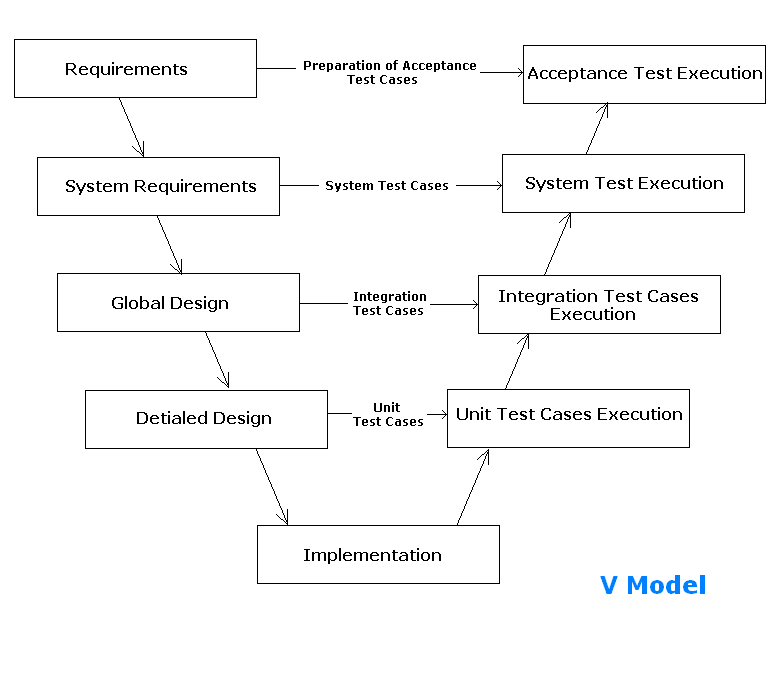
\includegraphics[width=0.9\linewidth]{../img/v-model}
		\caption[V Model]{}
		\label{fig:v-model}
	\end{figure}
	
	\subsubsection{Livelli di testing}
	Sono descritte nel seguito i vari livelli di test del modello adottato, le relative caratteristiche e la relativa funzione all'interno del sistema di test. 
	
	\paragraph{Test di validazione} si attua sul sistema completo per verificare che le funzionalità previste in fase di analisi siano effettivamente raggiunte da quest'ultimo. Le funzionalità testate sono quelle previste per l'utente finale.
	
	\paragraph{Test di Sistema} si attua sul sistema completamente integrato per verificare che i requisiti siano effettivamente soddisfatti.
	
	\paragraph{Test di Integrazione} è finalizzato alla verifica dell'interazione tra le componenti del sistema. Il soddisfacimento dei test di integrazione è essenziale ad assicurare che ogni parte del sistema non presenti errori dopo la fase di integrazione delle varie componenti.
	
	\paragraph{Test di Unità} è finalizzato alla verifica delle funzionalità di una ristretta parte di codice, solitamente una funzione o procedura. Spesso coprono anche la verifica dei costruttori delle classi.
	
	\subsubsection{Struttura del sistema di testing}
	La struttura del sistema di \mgls{testing} deve essere conforme alla struttura del sistema. Tale caratteristica è essenziale per il garantire il funzionamento dell'intero apparato di test. L'esecuzione dei test deve seguire l'ordine cronologico seguente:
	
	\begin{enumerate}
		\item Esecuzione e superamento dei test di unità;
		\item Esecuzione e superamento dei test di integrazione;
		\item Esecuzione e superamento dei test di sistema;
		\item Esecuzione e superamento dei test di \mgls{validazione}.
	\end{enumerate}
	
	E' cruciale per l'efficacia dei test che le componenti prodotti non entrino nella fase di test successiva, rispetto a quelle precedentemente esposte, se non soddisfa i test nel punto precedente.
	
	\subsubsection{Strategia di pianificazione}
	La pianificazione dei test deve essere preventiva rispetto alla produzione delle componenti oggetto di tali test. Pertanto si raccomanda che, non appena le informazioni ricavate tramite la \mgls{progettazione} lo permettano, vengano definiti i test riguardanti le componenti interessate.
	Pertanto, poiché la definizione dei test deve integrarsi con le varie fasi di \mgls{progettazione}, questa deve rispettare la seguente successione temporale:
	
	\begin{enumerate}
		\item definizione dei test di \mgls{validazione}  in periodo di \FA;
		\item definizione dei test di sistema in periodo di \FAD;
		\item definizione dei test di integrazione in periodo di \FPA;
		\item definizione dei test di unità in fase di \FPD.
	\end{enumerate}
	
	Si raccomanda, durante la definizione dei test, di utilizzare sistemi di gestione e archiviazione di questi ultimi che siano adeguati allo scopo e che ne facilitino la relativa gestione. E' inoltre essenziale mantenere il collegamento tra il test definito e lo scopo che ne motiva la definizione, sia esso un requisito del sistema o una sua componente o metodo. Anche tale caratteristica dovrebbe essere il più possibile automatizzata per mantenere e garantire in modo facile ed efficace la correttezza e consistenza dell'apparato di \mgls{testing}.
	
	\subsection{Test di Validazione}\label{test_pianificazione}
	\subsubsection{Descrizione dettagliata}
	\hypertarget{TV1}{}
	\paragraph{Test TV1}
	Verifica che l'ospite sia in grado di effettuare la registrazione presso il sistema attraverso i seguenti passi:
	
	\begin{enumerate}
		\item accesso alla pagina di registrazione;
		\item immissione dei dati dell'utente;
		\item conferma registrazione.
	\end{enumerate}
	\hypertarget{TV2}{}
	\paragraph{Test TV2}
	Verifica che l'ospite sia in grado di effettuare l'accesso attraverso i passi seguenti:
	
	\begin{enumerate}
		\item accesso alla pagina di login;
		\item inserimento credenziali;
		\item conferma accesso.
	\end{enumerate}
	\hypertarget{TV3}{}
	\paragraph{Test TV3}
	Verifica che uno studente sia in grado di eseguire un questionario attraverso i seguenti passi:
	
	\begin{enumerate}
		\item ricerca questionario;
		\item selezione questionario;
		\item compilazione questionario;
		\item conferma compilazione;
		\item visualizzazione dei risultati.
	\end{enumerate}
	\hypertarget{TV4}{}
	\paragraph{Test TV4}
	Verifica che il docente sia in grado di creare una domanda attraverso i seguenti passi:
	
	\begin{enumerate}
		\item accesso alla pagina di creazione domanda;
		\item scrittura della domanda in QML;
		\item selezione degli argomenti relativi alla domanda;
		\item conferma della creazione della domanda.
	\end{enumerate}
	\hypertarget{TV5}{}
	\paragraph{Test TV5}
	Verifica che il docente sia in grado di modificare una domanda attraverso i seguenti passi:
	
	\begin{enumerate}
		\item selezione domanda da modificare;
		\item modifica QML domanda;
		\item modifica argomenti domanda;
		\item conferma modifica.
	\end{enumerate}
	\hypertarget{TV6}{}
	\paragraph{Test TV6}
	Verifica che un docente sia in grado di cancellare una propria domanda non utilizzata da alcun questionario attraverso i seguenti passi:
	
	\begin{enumerate}
		\item selezione domanda da eliminare;
		\item conferma eliminazione domanda.
	\end{enumerate}
	\hypertarget{TV7}{}
	\paragraph{Test TV7}
	Verifica che un docente sia in grado di creare un questionario attraverso i seguenti passi:
	
	\begin{enumerate}
		\item accesso alla pagina di creazione questionario;
		\item selezione argomenti questionario;
		\item aggiunta domande questionario;
		\item conferma creazione.
	\end{enumerate}
	\hypertarget{TV8}{}
	\paragraph{Test TV8}
	Verifica che un docente sia in grado di modificare un proprio questionario attraverso i seguenti passi:
	
	\begin{enumerate}
		\item selezione questionario da modificare;
		\item modifica argomenti del questionario;
		\item modifica lista domande del questionario;
		\item conferma modifica.
	\end{enumerate}
	\hypertarget{TV9}{}
	\paragraph{Test TV9}
	Verifica che un docente sia in grado di eliminare un proprio questionario attraverso i seguenti passi:
	
	\begin{enumerate}
		\item selezione questionario;
		\item conferma eliminazione questionario.
	\end{enumerate}
	\hypertarget{TV10}{}
	\paragraph{Test TV10}
	Verifica che il docente sia in grado di creare un nuovo argomento attraverso i seguenti passi:
	
	\begin{enumerate}
		\item accesso pagina di aggiunta argomento;
		\item definizione dati argomento;
		\item conferma creazione argomento.
	\end{enumerate}
	\hypertarget{TV11}{}
	\paragraph{Test TV11}
	Verifica che un docente sia in grado di modificare un argomento attraverso i seguenti passi:
	
	\begin{enumerate}
		\item selezione argomento da modificare;
		\item modifica dati argomento;
		\item conferma modifica dati argomento.
	\end{enumerate}
	\hypertarget{TV12}{}
	\paragraph{Test TV12}
	Verifica che un docente sia in grado di eliminare un argomento attraverso i seguenti passi:
	
	\begin{enumerate}
		\item selezione argomento da eliminare;
		\item conferma eliminazione argomento.
	\end{enumerate}
	\hypertarget{TV13}{}
	\paragraph{Test TV13}
	Verifica che un amministratore o proprietario sia in grado di eliminare un utente di ruolo inferiore al proprio attraverso i seguenti passi:
	
	\begin{enumerate}
		\item selezione utente da eliminare;
		\item conferma eliminazione utente.
	\end{enumerate}
	\hypertarget{TV14}{}
	\paragraph{Test TV14}
	Verifica che un amministratore o proprietario sia in grado di cambiare il ruolo di un utente di ruolo inferiore al proprio attraverso i seguenti passi:
	
	\begin{enumerate}
		\item selezione utente;
		\item selezione ruolo utente;
		\item conferma modifica ruolo utente.
	\end{enumerate}
	\hypertarget{TV15}{}
	\paragraph{Test TV15}
	Verifica che un utente sia in grado di aggiornare i propri dati personali attraverso i seguenti passi:
	
	\begin{enumerate}
		\item accesso profilo utente;
		\item accesso pagina di modifica profilo;
		\item modifica dati personali;
		\item conferma modifica.
	\end{enumerate}
	\hypertarget{TV16}{}
	\paragraph{Test TV16}
	Verifica che un utente sia in grado di modificare la propria password attraverso i seguenti passi:
	
	\begin{enumerate}
		\item accesso profilo;
		\item selezione modifica password;
		\item inserimento vecchia password;
		\item inserimento nuova password;
		\item inserimento nuova password una seconda volta;
		\item conferma modifica password.
	\end{enumerate}
	\hypertarget{TV17}{}
	\paragraph{Test TV17}
	Verifica che un utente sia in grado di disconnettersi dal sistema attraverso i seguenti passi:
	
	\begin{enumerate}
		\item accesso profilo;
		\item conferma disconnessione.
	\end{enumerate}
	\hypertarget{TV18}{}
	\paragraph{Test TV18}
	Verifica che un amministratore o proprietario sia in grado di visualizzare la lista degli utenti, eventualmente specificando parametri per il filtraggio del risultati, attraverso i seguenti passi:
	
	\begin{enumerate}
		\item accesso lista utenti;
		\item specifica parametri di filtraggio dei risultati;
		\item visualizzazione elenco.
	\end{enumerate}
	\hypertarget{TV19}{}
	\paragraph
	Verifica che un docente sia in grado di visualizzare la lista degli argomenti, eventualmente specificando parametri per il filtraggio del risultati, attraverso i seguenti passi:
	
	\begin{enumerate}
		\item accesso lista argomenti;
		\item specifica parametri di filtraggio dei risultati;
		\item visualizzazione elenco.
	\end{enumerate}
	\hypertarget{TV20}{}
	\paragraph{Test TV20}
	Verifica che un docente sia in grado di visualizzare la lista delle domande, eventualmente specificando parametri per il filtraggio del risultati, attraverso i seguenti passi:
	
	\begin{enumerate}
		\item accesso lista domande;
		\item specifica parametri di filtraggio dei risultati;
		\item visualizzazione elenco.
	\end{enumerate}
	\hypertarget{TV21}{}
	\paragraph{Test TV21}
	Verifica che un utente sia in grado di visualizzare la lista dei questionari, eventualmente specificando parametri per il filtraggio del risultati, attraverso i seguenti passi:
	
	\begin{enumerate}
		\item accesso lista questionari;
		\item specifica parametri di filtraggio dei risultati;
		\item visualizzazione elenco.
	\end{enumerate}
	\hypertarget{TV22}{}
	\paragraph{Test TV22}
	Verifica che il docente sia in grado di visualizzare una domanda attraverso i passi seguenti: \begin{enumerate} \item selezione della domanda; \item visualizzazione dati domanda. \end{enumerate}
	\hypertarget{TV23}{}
	\paragraph{Test TV23}
	Verifica che il docente sia in grado di visualizzare un questionario attraverso i passi seguenti: \begin{enumerate} \item selezione del questionario; \item visualizzazione dati e elenco domande questionario. \end{enumerate}
	
	\subsubsection{Tracciamento TV-Requisito}
	\begin{longtable}{|r l|p{6cm}|l|l|}
		\hline
		\multicolumn{2}{|c|}{Validazione} & Descrizione & Requisito & Stato\tabularnewline
		\hline
		& TV1 & Verifica che l'ospite sia in grado di effettuare la registrazione presso il sistema attraverso i seguenti passi:
		
		\begin{enumerate}
			\item accesso alla pagina di registrazione;
			\item immissione dei dati dell'utente;
			\item conferma registrazione.
		\end{enumerate} & R-3F9 & success\tabularnewline
		\hline
		& TV2 & Verifica che l'ospite sia in grado di effettuare l'accesso attraverso i passi seguenti:
		
		\begin{enumerate}
			\item accesso alla pagina di login;
			\item inserimento credenziali;
			\item conferma accesso.
		\end{enumerate} & R-3F31 & success\tabularnewline
		\hline
		& TV3 & Verifica che uno studente sia in grado di eseguire un questionario attraverso i seguenti passi:
		
		\begin{enumerate}
			\item ricerca questionario;
			\item selezione questionario;
			\item compilazione questionario;
			\item conferma compilazione;
			\item visualizzazione dei risultati.
		\end{enumerate} & R-3F16 & success\tabularnewline
		\hline
		& TV4 & Verifica che il docente sia in grado di creare una domanda attraverso i seguenti passi:
		
		\begin{enumerate}
			\item accesso alla pagina di creazione domanda;
			\item scrittura della domanda in QML;
			\item selezione degli argomenti relativi alla domanda;
			\item conferma della creazione della domanda.
		\end{enumerate} & R-3F7.11.1 & success\tabularnewline
		\hline
		& TV5 & Verifica che il docente sia in grado di modificare una domanda attraverso i seguenti passi:
		
		\begin{enumerate}
			\item selezione domanda da modificare;
			\item modifica QML domanda;
			\item modifica argomenti domanda;
			\item conferma modifica.
		\end{enumerate} & R-3F7.11.2 & success\tabularnewline
		\hline
		& TV6 & Verifica che un docente sia in grado di cancellare una propria domanda non utilizzata da alcun questionario attraverso i seguenti passi:
		
		\begin{enumerate}
			\item selezione domanda da eliminare;
			\item conferma eliminazione domanda.
		\end{enumerate} & R-3F7.11.3 & success\tabularnewline
		\hline
		& TV7 & Verifica che un docente sia in grado di creare un questionario attraverso i seguenti passi:
		
		\begin{enumerate}
			\item accesso alla pagina di creazione questionario;
			\item selezione argomenti questionario;
			\item aggiunta domande questionario;
			\item conferma creazione.
		\end{enumerate} & R-3F7.7 & success\tabularnewline
		\hline
		& TV8 & Verifica che un docente sia in grado di modificare un proprio questionario attraverso i seguenti passi:
		
		\begin{enumerate}
			\item selezione questionario da modificare;
			\item modifica argomenti del questionario;
			\item modifica lista domande del questionario;
			\item conferma modifica.
		\end{enumerate} & R-3F7.12 & success\tabularnewline
		\hline
		& TV9 & Verifica che un docente sia in grado di eliminare un proprio questionario attraverso i seguenti passi:
		
		\begin{enumerate}
			\item selezione questionario;
			\item conferma eliminazione questionario.
		\end{enumerate} & R-3F7.13 & success\tabularnewline
		\hline
		& TV10 & Verifica che il docente sia in grado di creare un nuovo argomento attraverso i seguenti passi:
		
		\begin{enumerate}
			\item accesso pagina di aggiunta argomento;
			\item definizione dati argomento;
			\item conferma creazione argomento.
		\end{enumerate} & R-3F22.1 & success\tabularnewline
		\hline
		& TV11 & Verifica che un docente sia in grado di modificare un argomento attraverso i seguenti passi:
		
		\begin{enumerate}
			\item selezione argomento da modificare;
			\item modifica dati argomento;
			\item conferma modifica dati argomento.
		\end{enumerate} & R-3F22.3 & success\tabularnewline
		\hline
		& TV12 & Verifica che un docente sia in grado di eliminare un argomento attraverso i seguenti passi:
		
		\begin{enumerate}
			\item selezione argomento da eliminare;
			\item conferma eliminazione argomento.
		\end{enumerate} & R-3F22.2 & success\tabularnewline
		\hline
		& TV13 & Verifica che un amministratore o proprietario sia in grado di eliminare un utente di ruolo inferiore al proprio attraverso i seguenti passi:
		
		\begin{enumerate}
			\item selezione utente da eliminare;
			\item conferma eliminazione utente.
		\end{enumerate} & R-3F11.2 & success\tabularnewline
		\hline
		& TV14 & Verifica che un amministratore o proprietario sia in grado di cambiare il ruolo di un utente di ruolo inferiore al proprio attraverso i seguenti passi:
		
		\begin{enumerate}
			\item selezione utente;
			\item selezione ruolo utente;
			\item conferma modifica ruolo utente.
		\end{enumerate} & R-3F11.1 & success\tabularnewline
		\hline
		& TV15 & Verifica che un utente sia in grado di aggiornare i propri dati personali attraverso i seguenti passi:
		
		\begin{enumerate}
			\item accesso profilo utente;
			\item accesso pagina di modifica profilo;
			\item modifica dati personali;
			\item conferma modifica.
		\end{enumerate} & R-3F13.3 & success\tabularnewline
		\hline
		& TV16 & Verifica che un utente sia in grado di modificare la propria password attraverso i seguenti passi:
		
		\begin{enumerate}
			\item accesso profilo;
			\item selezione modifica password;
			\item inserimento vecchia password;
			\item inserimento nuova password;
			\item inserimento nuova password una seconda volta;
			\item conferma modifica password.
		\end{enumerate} & R-3F13.2 & success\tabularnewline
		\hline
		& TV17 & Verifica che un utente sia in grado di disconnettersi dal sistema attraverso i seguenti passi:
		
		\begin{enumerate}
			\item accesso profilo;
			\item conferma disconnessione.
		\end{enumerate} & R-3F17 & success\tabularnewline
		\hline
		& TV18 & Verifica che un amministratore o proprietario sia in grado di visualizzare la lista degli utenti, eventualmente specificando parametri per il filtraggio del risultati, attraverso i seguenti passi:
		
		\begin{enumerate}
			\item accesso lista utenti;
			\item specifica parametri di filtraggio dei risultati;
			\item visualizzazione elenco.
		\end{enumerate} & R-3F32 & success\tabularnewline
		\hline
		& TV19 & Verifica che un docente sia in grado di visualizzare la lista degli argomenti, eventualmente specificando parametri per il filtraggio del risultati, attraverso i seguenti passi:
		
		\begin{enumerate}
			\item accesso lista argomenti;
			\item specifica parametri di filtraggio dei risultati;
			\item visualizzazione elenco.
		\end{enumerate} & R-3F22.4 & success\tabularnewline
		\hline
		& TV20 & Verifica che un docente sia in grado di visualizzare la lista delle domande, eventualmente specificando parametri per il filtraggio del risultati, attraverso i seguenti passi:
		
		\begin{enumerate}
			\item accesso lista domande;
			\item specifica parametri di filtraggio dei risultati;
			\item visualizzazione elenco.
		\end{enumerate} & R-3F19 & success\tabularnewline
		\hline
		& TV21 & Verifica che un utente sia in grado di visualizzare la lista dei questionari, eventualmente specificando parametri per il filtraggio del risultati, attraverso i seguenti passi:
		
		\begin{enumerate}
			\item accesso lista questionari;
			\item specifica parametri di filtraggio dei risultati;
			\item visualizzazione elenco.
		\end{enumerate} & R-3F14 & success\tabularnewline
		\hline
		& TV22 & Verifica che il docente sia in grado di visualizzare una domanda attraverso i passi seguenti: \begin{enumerate} \item selezione della domanda; \item visualizzazione dati domanda. \end{enumerate} & R-3F29 & success\tabularnewline
		\hline
		& TV23 & Verifica che il docente sia in grado di visualizzare un questionario attraverso i passi seguenti: \begin{enumerate} \item selezione del questionario; \item visualizzazione dati e elenco domande questionario. \end{enumerate} & R-3F30 & success\tabularnewline
		\hline
		\caption{Tabella test validazione / requisiti} \tabularnewline
	\end{longtable}
	\subsection{Test di Sistema}\label{test_sistema}
	\subsubsection{Descrizione dettagliata }
	\begin{longtable}{|l|p{6cm}|l|l|}
		\hline
		Test & Descrizione & Stato & Requisito\tabularnewline
		\hline
		TS7.5 & I sotto-requisiti obbligatori sono verificati e viene verificato che il QML riesca a descrivere in maniera efficace tutte le caratteristiche previste per un questionario e le relative domande & success & \hypertarget{R-3F7.5}{R-3F7.5}\tabularnewline
		\hline
		TS7.5.1 & I sotto-requisiti obbligatori sono verificati e viene verificato che il QML permetta di definire il testo di una domanda e delle relative risposte attraverso una sintassi univoca & success & \hypertarget{R-3F7.5.1}{R-3F7.5.1}\tabularnewline
		\hline
		TS7.5.1.2 & Viene verificato che il QML permetta l'inserimento di immagini & success & \hypertarget{R-3F7.5.1.2}{R-3F7.5.1.2}\tabularnewline
		\hline
		TS7.5.1.6 & Viene verificato che il QML permetta di definire vari tipi di domanda & success & \hypertarget{R-3F7.5.1.6}{R-3F7.5.1.6}\tabularnewline
		\hline
		TS7.5.3 & Viene verificato che le domande in QML possano essere scritte e modificate da un docente & success & \hypertarget{R-3F7.5.3}{R-3F7.5.3}\tabularnewline
		\hline
		TS7.5.5 & Viene verificato che Il QML possa gestire risposte vero/falso, risposte a scelta multipla, possa contenere testi e immagini	 & success & \hypertarget{R-3F7.5.5}{R-3F7.5.5}\tabularnewline
		\hline
		TS7.7 & Viene verificato che un docente possa costruire un nuovo questionario utilizzando le domande presenti nel sistema e che non sia possibile creare un questionario che non contenga domande o argomenti
		& success & \hypertarget{R-3F7.7}{R-3F7.7}\tabularnewline
		\hline
		TS7.11 & Viene verificato che sia possibile per un docente eseguire le operazioni di inserimento, modifica e rimozione di una domanda e che tutti i casi non corretti vengano segnalati & success & \hypertarget{R-3F7.11}{R-3F7.11}\tabularnewline
		\hline
		TS7.11.1.2.1 & Viene verificato che il sistema sia in grado di verificare l'inserimento di QML valido e, in caso contrario, segnalare un errore & success & \hypertarget{R-3F7.11.1.2.1}{R-3F7.11.1.2.1}\tabularnewline
		\hline
		TS7.11.1.2.2 & Viene verificato che il docente possa inserire domande di tipo vero/falso	 & success & \hypertarget{R-3F7.11.1.2.2}{R-3F7.11.1.2.2}\tabularnewline
		\hline
		TS7.11.1.2.4 & Viene verificato che il docente possa inserire domande di tipo scelta multipla & success & \hypertarget{R-1F7.11.1.2.4}{R-1F7.11.1.2.4}\tabularnewline
		\hline
		TS7.12 & Viene verificato che sia possibile per un docente modificare un questionario che ha precedentemente creato & success & \hypertarget{R-3F7.12}{R-3F7.12}\tabularnewline
		\hline
		TS7.13 & Viene verificato che sia possibile per un docente eliminare un questionario che ha precedentemente creato & success & \hypertarget{R-3F7.13}{R-3F7.13}\tabularnewline
		\hline
		TS8 & Viene verificato che il sistema possa gestire l'accesso e la registrazione di ogni tipo di utente previsto & success & \hypertarget{R-3F8}{R-3F8}\tabularnewline
		\hline
		TS9 & Viene verificato che sia possibile per ogni tipo di utente registrarsi presso il sistema & success & \hypertarget{R-3F9}{R-3F9}\tabularnewline
		\hline
		TS9.1 & Viene verificato che il sistema consenta le funzionalità utente solo se possiede un proprietario & success & \hypertarget{R-3F9.1}{R-3F9.1}\tabularnewline
		\hline
		TS9.2 & I sotto-requisiti sono verificati. Viene verificato che sia possibile per un utente registrarsi presso il sistema con una password e le proprie informazioni personali & success & \hypertarget{R-3F9.2}{R-3F9.2}\tabularnewline
		\hline
		TS9.2.1 & Viene verificato che il sistema segnali un errore se non vengono inseriti tutti i campi necessari alla registrazione di un utente & success & \hypertarget{R-3F9.2.1}{R-3F9.2.1}\tabularnewline
		\hline
		TS11 & Viene verificato che il sistema gestisca correttamente tutte le funzionalità di un amministratore & success & \hypertarget{R-3F11}{R-3F11}\tabularnewline
		\hline
		TS13 & Viene verificato che il sistema consenta ad un utente di modificare le proprie informazioni personali presenti nel sistema & success & \hypertarget{R-3F13}{R-3F13}\tabularnewline
		\hline
		TS14 & Viene verificato che, per ogni tipo di utente, il sistema gestisca correttamente la ricerca di un questionario da parte di un utente & success & \hypertarget{R-3F14}{R-3F14}\tabularnewline
		\hline
		TS16 & Viene verificato che un utente sia in grado di rispondere alle domande di un questionario & success & \hypertarget{R-3F16}{R-3F16}\tabularnewline
		\hline
		TS17 & Viene verificato che per un qualsiasi tipo di utente autenticato presso il sistema sia possibile effettuare correttamente il log-out  & success & \hypertarget{R-3F17}{R-3F17}\tabularnewline
		\hline
		TS18 & Viene verificato che il sistema consenta e gestisca correttamente tutte le azioni previste per il proprietario & success & \hypertarget{R-3F18}{R-3F18}\tabularnewline
		\hline
		TS19 & Viene verificato che per un docente sia possibile effettuare correttamente la ricerca di una domanda presente nel sistema & success & \hypertarget{R-3F19}{R-3F19}\tabularnewline
		\hline
		TS22 & Viene verificato che sia possibile per un docente, amministratore e proprietario la gestione degli argomenti presenti nel sistema & success & \hypertarget{R-3F22}{R-3F22}\tabularnewline
		\hline
		TS29 & Viene verificato che il sistema consenta ad un docente di visualizzare una domanda & success & \hypertarget{R-3F29}{R-3F29}\tabularnewline
		\hline
		TS30 & Viene verificato che il sistema consenta ad un docente di visualizzare un questionario & success & \hypertarget{R-3F30}{R-3F30}\tabularnewline
		\hline
		\caption{Tabella di tracciamento test di sistema / requisiti} \tabularnewline
	\end{longtable}
	\subsubsection{Tracciamento TS-Requisito}
	\begin{longtable}{|r l|l|}
		\hline
		\multicolumn{2}{|c|}{Requisito} & Test\tabularnewline
		\hline
		& R-3V1 & Il resposabile certifica questo requisito\tabularnewline
		\hline
		& R-3V2 & Il resposabile certifica questo requisito\tabularnewline
		\hline
		& R-3V3 & Validatore w3c\tabularnewline
		\hline
		\begin{tikzpicture}
		\draw [->, thick] (0.2,0.2) -- (0.2,0.1) -- (1,0.1);
		\end{tikzpicture} & R-3V3.1 & test prodotto su browser specificato\tabularnewline
		\hline
		\begin{tikzpicture}
		\draw [->, thick] (0.2,0.2) -- (0.2,0.1) -- (1,0.1);
		\end{tikzpicture} & R-3V3.2 & Validatore w3c\tabularnewline
		\hline
		\begin{tikzpicture}
		\draw [->, thick] (0.2,0.2) -- (0.2,0.1) -- (1,0.1);
		\end{tikzpicture} & R-3V3.3 & test prodotto su browser specificato\tabularnewline
		\hline
		\begin{tikzpicture}
		\draw [->, thick] (0.2,0.2) -- (0.2,0.1) -- (1,0.1);
		\end{tikzpicture} & R-3V3.4 & I moduli superano test unità, verifica use cases relativi\tabularnewline
		\hline
		& R-3V4 & Il resposabile certifica questo requisito\tabularnewline
		\hline
		& R-3V5 & Il resposabile certifica questo requisito\tabularnewline
		\hline
		& R-3V6 & Il sistema utilizza tecnologie supportate su tali dispositivi\tabularnewline
		\hline
		\begin{tikzpicture}
		\draw [->, thick] (0.2,0.2) -- (0.2,0.1) -- (1,0.1);
		\end{tikzpicture} & R-3V6.1 & Il sistema utilizza tecnologie supportate su tali dispositivi\tabularnewline
		\hline
		\begin{tikzpicture}
		\draw [->, thick] (0.2,0.2) -- (0.2,0.1) -- (1,0.1);
		\end{tikzpicture} & R-3V6.2 & Il sistema utilizza tecnologie supportate su tali dispositivi\tabularnewline
		\hline
		& R-3F7 & I moduli superano test unità, verifica use cases relativi\tabularnewline
		\hline
		\begin{tikzpicture}
		\draw [->, thick] (0.2,0.2) -- (0.2,0.1) -- (1,0.1);
		\end{tikzpicture} & R-3F7.1 & I moduli superano test unità, verifica use cases relativi\tabularnewline
		\hline
		\begin{tikzpicture}
		\draw [->, thick] (0.2,0.2) -- (0.2,0.1) -- (1,0.1);
		\end{tikzpicture} & R-3F7.2 & I moduli superano test unità, verifica use cases relativi\tabularnewline
		\hline
		\begin{tikzpicture}
		\draw [->, thick] (0.2,0.2) -- (0.2,0.1) -- (1,0.1);
		\end{tikzpicture} & R-3F7.3 & I moduli superano test unità, verifica use cases relativi\tabularnewline
		\hline
		\begin{tikzpicture}
		\draw [->, thick] (0.2,0.2) -- (0.2,0.1) -- (1,0.1);
		\end{tikzpicture} & R-3F7.4 & I moduli superano test unità, verifica use cases relativi\tabularnewline
		\hline
		\begin{tikzpicture}
		\draw [->, thick] (0.2,0.2) -- (0.2,0.1) -- (1,0.1);
		\end{tikzpicture} & R-3F7.5 & TS7.5\tabularnewline
		\hline
		\begin{tikzpicture}
		\draw [->, thick] (0.4,0.2) -- (0.4,0.1) -- (1,0.1);
		\end{tikzpicture} & R-3F7.5.1 & TS7.5.1\tabularnewline
		\hline
		\begin{tikzpicture}
		\draw [->, thick] (0.6,0.2) -- (0.6,0.1) -- (1,0.1);
		\end{tikzpicture} & R-2F7.5.1.1 & I moduli superano test unità, verifica use cases relativi\tabularnewline
		\hline
		\begin{tikzpicture}
		\draw [->, thick] (0.6,0.2) -- (0.6,0.1) -- (1,0.1);
		\end{tikzpicture} & R-3F7.5.1.2 & TS7.5.1.2\tabularnewline
		\hline
		\begin{tikzpicture}
		\draw [->, thick] (0.6,0.2) -- (0.6,0.1) -- (1,0.1);
		\end{tikzpicture} & R-2F7.5.1.3 & I moduli superano test unità, verifica use cases relativi\tabularnewline
		\hline
		\begin{tikzpicture}
		\draw [->, thick] (0.6,0.2) -- (0.6,0.1) -- (1,0.1);
		\end{tikzpicture} & R-2F7.5.1.4 & I moduli superano test unità, verifica use cases relativi\tabularnewline
		\hline
		\begin{tikzpicture}
		\draw [->, thick] (0.6,0.2) -- (0.6,0.1) -- (1,0.1);
		\end{tikzpicture} & R-2F7.5.1.5 & I moduli superano test unità, verifica use cases relativi\tabularnewline
		\hline
		\begin{tikzpicture}
		\draw [->, thick] (0.6,0.2) -- (0.6,0.1) -- (1,0.1);
		\end{tikzpicture} & R-3F7.5.1.6 & TS7.5.1.6\tabularnewline
		\hline
		\begin{tikzpicture}
		\draw [->, thick] (0.6,0.2) -- (0.6,0.1) -- (1,0.1);
		\end{tikzpicture} & R-2F7.5.1.7 & I moduli superano test unità, verifica use cases relativi\tabularnewline
		\hline
		\begin{tikzpicture}
		\draw [->, thick] (0.6,0.2) -- (0.6,0.1) -- (1,0.1);
		\end{tikzpicture} & R-2F7.5.1.8 & I moduli superano test unità, verifica use cases relativi\tabularnewline
		\hline
		\begin{tikzpicture}
		\draw [->, thick] (0.4,0.2) -- (0.4,0.1) -- (1,0.1);
		\end{tikzpicture} & R-2F7.5.2 & I moduli superano test unità, verifica use cases relativi\tabularnewline
		\hline
		\begin{tikzpicture}
		\draw [->, thick] (0.4,0.2) -- (0.4,0.1) -- (1,0.1);
		\end{tikzpicture} & R-3F7.5.3 & TS7.5.3\tabularnewline
		\hline
		\begin{tikzpicture}
		\draw [->, thick] (0.4,0.2) -- (0.4,0.1) -- (1,0.1);
		\end{tikzpicture} & R-2F7.5.4 & I moduli superano test unità, verifica use cases relativi\tabularnewline
		\hline
		\begin{tikzpicture}
		\draw [->, thick] (0.4,0.2) -- (0.4,0.1) -- (1,0.1);
		\end{tikzpicture} & R-3F7.5.5 & TS7.5.5\tabularnewline
		\hline
		\begin{tikzpicture}
		\draw [->, thick] (0.2,0.2) -- (0.2,0.1) -- (1,0.1);
		\end{tikzpicture} & R-2F7.6 & I moduli superano test unità, verifica use cases relativi\tabularnewline
		\hline
		\begin{tikzpicture}
		\draw [->, thick] (0.2,0.2) -- (0.2,0.1) -- (1,0.1);
		\end{tikzpicture} & R-3F7.7 & TS7.7\tabularnewline
		\hline
		\begin{tikzpicture}
		\draw [->, thick] (0.4,0.2) -- (0.4,0.1) -- (1,0.1);
		\end{tikzpicture} & R-3F7.7.1 & I moduli superano test unità, verifica use cases relativi\tabularnewline
		\hline
		\begin{tikzpicture}
		\draw [->, thick] (0.2,0.2) -- (0.2,0.1) -- (1,0.1);
		\end{tikzpicture} & R-2F7.8 & I moduli superano test unità, verifica use cases relativi\tabularnewline
		\hline
		\begin{tikzpicture}
		\draw [->, thick] (0.2,0.2) -- (0.2,0.1) -- (1,0.1);
		\end{tikzpicture} & R-2F7.9 & I moduli superano test unità, verifica use cases relativi\tabularnewline
		\hline
		\begin{tikzpicture}
		\draw [->, thick] (0.2,0.2) -- (0.2,0.1) -- (1,0.1);
		\end{tikzpicture} & R-2F7.10 & I moduli superano test unità, verifica use cases relativi\tabularnewline
		\hline
		\begin{tikzpicture}
		\draw [->, thick] (0.4,0.2) -- (0.4,0.1) -- (1,0.1);
		\end{tikzpicture} & R-2F7.10.1 & I moduli superano test unità, verifica use cases relativi\tabularnewline
		\hline
		\begin{tikzpicture}
		\draw [->, thick] (0.4,0.2) -- (0.4,0.1) -- (1,0.1);
		\end{tikzpicture} & R-2F7.10.2 & I moduli superano test unità, verifica use cases relativi\tabularnewline
		\hline
		\begin{tikzpicture}
		\draw [->, thick] (0.4,0.2) -- (0.4,0.1) -- (1,0.1);
		\end{tikzpicture} & R-2F7.10.3 & I moduli superano test unità, verifica use cases relativi\tabularnewline
		\hline
		\begin{tikzpicture}
		\draw [->, thick] (0.2,0.2) -- (0.2,0.1) -- (1,0.1);
		\end{tikzpicture} & R-3F7.11 & TS7.11\tabularnewline
		\hline
		\begin{tikzpicture}
		\draw [->, thick] (0.4,0.2) -- (0.4,0.1) -- (1,0.1);
		\end{tikzpicture} & R-3F7.11.1 & I moduli superano test unità, verifica use cases relativi\tabularnewline
		\hline
		\begin{tikzpicture}
		\draw [->, thick] (0.6,0.2) -- (0.6,0.1) -- (1,0.1);
		\end{tikzpicture} & R-3F7.11.1.1 & I moduli superano test unità, verifica use cases relativi\tabularnewline
		\hline
		\begin{tikzpicture}
		\draw [->, thick] (0.8,0.2) -- (0.8,0.1) -- (1,0.1);
		\end{tikzpicture} & R-3F7.11.1.1.1 & I moduli superano test unità, verifica use cases relativi\tabularnewline
		\hline
		\begin{tikzpicture}
		\draw [->, thick] (0.6,0.2) -- (0.6,0.1) -- (1,0.1);
		\end{tikzpicture} & R-3F7.11.1.2 & I moduli superano test unità, verifica use cases relativi\tabularnewline
		\hline
		\begin{tikzpicture}
		\draw [->, thick] (0.8,0.2) -- (0.8,0.1) -- (1,0.1);
		\end{tikzpicture} & R-3F7.11.1.2.1 & TS7.11.1.2.1\tabularnewline
		\hline
		\begin{tikzpicture}
		\draw [->, thick] (0.8,0.2) -- (0.8,0.1) -- (1,0.1);
		\end{tikzpicture} & R-3F7.11.1.2.2 & TS7.11.1.2.2\tabularnewline
		\hline
		\begin{tikzpicture}
		\draw [->, thick] (0.8,0.2) -- (0.8,0.1) -- (1,0.1);
		\end{tikzpicture} & R-3F7.11.1.2.3 & I moduli superano test unità, verifica use cases relativi\tabularnewline
		\hline
		\begin{tikzpicture}
		\draw [->, thick] (0.8,0.2) -- (0.8,0.1) -- (1,0.1);
		\end{tikzpicture} & R-1F7.11.1.2.4 & TS7.11.1.2.4\tabularnewline
		\hline
		\begin{tikzpicture}
		\draw [->, thick] (0.8,0.2) -- (0.8,0.1) -- (1,0.1);
		\end{tikzpicture} & R-1F7.11.1.2.5 & I moduli superano test unità, verifica use cases relativi\tabularnewline
		\hline
		\begin{tikzpicture}
		\draw [->, thick] (0.8,0.2) -- (0.8,0.1) -- (1,0.1);
		\end{tikzpicture} & R-1F7.11.1.2.6 & I moduli superano test unità, verifica use cases relativi\tabularnewline
		\hline
		\begin{tikzpicture}
		\draw [->, thick] (0.8,0.2) -- (0.8,0.1) -- (1,0.1);
		\end{tikzpicture} & R-2F7.11.1.2.7 & I moduli superano test unità, verifica use cases relativi\tabularnewline
		\hline
		\begin{tikzpicture}
		\draw [->, thick] (0.4,0.2) -- (0.4,0.1) -- (1,0.1);
		\end{tikzpicture} & R-3F7.11.2 & I moduli superano test unità, verifica use cases relativi\tabularnewline
		\hline
		\begin{tikzpicture}
		\draw [->, thick] (0.4,0.2) -- (0.4,0.1) -- (1,0.1);
		\end{tikzpicture} & R-3F7.11.3 & I moduli superano test unità, verifica use cases relativi\tabularnewline
		\hline
		\begin{tikzpicture}
		\draw [->, thick] (0.2,0.2) -- (0.2,0.1) -- (1,0.1);
		\end{tikzpicture} & R-3F7.12 & TS7.12\tabularnewline
		\hline
		\begin{tikzpicture}
		\draw [->, thick] (0.4,0.2) -- (0.4,0.1) -- (1,0.1);
		\end{tikzpicture} & R-3F7.12.1 & I moduli superano test unità, verifica use cases relativi\tabularnewline
		\hline
		\begin{tikzpicture}
		\draw [->, thick] (0.4,0.2) -- (0.4,0.1) -- (1,0.1);
		\end{tikzpicture} & R-3F7.12.2 & I moduli superano test unità, verifica use cases relativi\tabularnewline
		\hline
		\begin{tikzpicture}
		\draw [->, thick] (0.4,0.2) -- (0.4,0.1) -- (1,0.1);
		\end{tikzpicture} & R-3F7.12.3 & I moduli superano test unità, verifica use cases relativi\tabularnewline
		\hline
		\begin{tikzpicture}
		\draw [->, thick] (0.4,0.2) -- (0.4,0.1) -- (1,0.1);
		\end{tikzpicture} & R-3F7.12.4 & I moduli superano test unità, verifica use cases relativi\tabularnewline
		\hline
		\begin{tikzpicture}
		\draw [->, thick] (0.2,0.2) -- (0.2,0.1) -- (1,0.1);
		\end{tikzpicture} & R-3F7.13 & TS7.13\tabularnewline
		\hline
		& R-3F8 & TS8\tabularnewline
		\hline
		& R-3F9 & TS9\tabularnewline
		\hline
		\begin{tikzpicture}
		\draw [->, thick] (0.2,0.2) -- (0.2,0.1) -- (1,0.1);
		\end{tikzpicture} & R-3F9.1 & TS9.1\tabularnewline
		\hline
		\begin{tikzpicture}
		\draw [->, thick] (0.2,0.2) -- (0.2,0.1) -- (1,0.1);
		\end{tikzpicture} & R-3F9.2 & TS9.2\tabularnewline
		\hline
		\begin{tikzpicture}
		\draw [->, thick] (0.4,0.2) -- (0.4,0.1) -- (1,0.1);
		\end{tikzpicture} & R-3F9.2.1 & TS9.2.1\tabularnewline
		\hline
		\begin{tikzpicture}
		\draw [->, thick] (0.4,0.2) -- (0.4,0.1) -- (1,0.1);
		\end{tikzpicture} & R-3F9.2.2 & I moduli superano test unità, verifica use cases relativi\tabularnewline
		\hline
		\begin{tikzpicture}
		\draw [->, thick] (0.2,0.2) -- (0.2,0.1) -- (1,0.1);
		\end{tikzpicture} & R-3F9.3 & I moduli superano test unità, verifica use cases relativi\tabularnewline
		\hline
		\begin{tikzpicture}
		\draw [->, thick] (0.2,0.2) -- (0.2,0.1) -- (1,0.1);
		\end{tikzpicture} & R-3F9.4 & I moduli superano test unità, verifica use cases relativi\tabularnewline
		\hline
		\begin{tikzpicture}
		\draw [->, thick] (0.2,0.2) -- (0.2,0.1) -- (1,0.1);
		\end{tikzpicture} & R-3F9.5 & I moduli superano test unità, verifica use cases relativi\tabularnewline
		\hline
		& R-3V10 & I moduli superano test unità, verifica use cases relativi\tabularnewline
		\hline
		& R-3F11 & TS11\tabularnewline
		\hline
		\begin{tikzpicture}
		\draw [->, thick] (0.2,0.2) -- (0.2,0.1) -- (1,0.1);
		\end{tikzpicture} & R-3F11.1 & I moduli superano test unità, verifica use cases relativi\tabularnewline
		\hline
		\begin{tikzpicture}
		\draw [->, thick] (0.2,0.2) -- (0.2,0.1) -- (1,0.1);
		\end{tikzpicture} & R-3F11.2 & I moduli superano test unità, verifica use cases relativi\tabularnewline
		\hline
		& R-2F12 & I moduli superano test unità, verifica use cases relativi\tabularnewline
		\hline
		\begin{tikzpicture}
		\draw [->, thick] (0.2,0.2) -- (0.2,0.1) -- (1,0.1);
		\end{tikzpicture} & R-2F12.1 & I moduli superano test unità, verifica use cases relativi\tabularnewline
		\hline
		\begin{tikzpicture}
		\draw [->, thick] (0.4,0.2) -- (0.4,0.1) -- (1,0.1);
		\end{tikzpicture} & R-2F12.1.1 & I moduli superano test unità, verifica use cases relativi\tabularnewline
		\hline
		\begin{tikzpicture}
		\draw [->, thick] (0.6,0.2) -- (0.6,0.1) -- (1,0.1);
		\end{tikzpicture} & R-2F12.1.1.1 & I moduli superano test unità, verifica use cases relativi\tabularnewline
		\hline
		\begin{tikzpicture}
		\draw [->, thick] (0.4,0.2) -- (0.4,0.1) -- (1,0.1);
		\end{tikzpicture} & R-2F12.1.2 & I moduli superano test unità, verifica use cases relativi\tabularnewline
		\hline
		\begin{tikzpicture}
		\draw [->, thick] (0.4,0.2) -- (0.4,0.1) -- (1,0.1);
		\end{tikzpicture} & R-2F12.1.3 & I moduli superano test unità, verifica use cases relativi\tabularnewline
		\hline
		\begin{tikzpicture}
		\draw [->, thick] (0.2,0.2) -- (0.2,0.1) -- (1,0.1);
		\end{tikzpicture} & R-2F12.2 & I moduli superano test unità, verifica use cases relativi\tabularnewline
		\hline
		\begin{tikzpicture}
		\draw [->, thick] (0.2,0.2) -- (0.2,0.1) -- (1,0.1);
		\end{tikzpicture} & R-2F12.3 & I moduli superano test unità, verifica use cases relativi\tabularnewline
		\hline
		\begin{tikzpicture}
		\draw [->, thick] (0.4,0.2) -- (0.4,0.1) -- (1,0.1);
		\end{tikzpicture} & R-2F12.3.1 & I moduli superano test unità, verifica use cases relativi\tabularnewline
		\hline
		\begin{tikzpicture}
		\draw [->, thick] (0.4,0.2) -- (0.4,0.1) -- (1,0.1);
		\end{tikzpicture} & R-2F12.3.2 & I moduli superano test unità, verifica use cases relativi\tabularnewline
		\hline
		\begin{tikzpicture}
		\draw [->, thick] (0.4,0.2) -- (0.4,0.1) -- (1,0.1);
		\end{tikzpicture} & R-2F12.3.3 & I moduli superano test unità, verifica use cases relativi\tabularnewline
		\hline
		& R-3F13 & TS13\tabularnewline
		\hline
		\begin{tikzpicture}
		\draw [->, thick] (0.2,0.2) -- (0.2,0.1) -- (1,0.1);
		\end{tikzpicture} & R-3F13.1 & I moduli superano test unità, verifica use cases relativi\tabularnewline
		\hline
		\begin{tikzpicture}
		\draw [->, thick] (0.4,0.2) -- (0.4,0.1) -- (1,0.1);
		\end{tikzpicture} & R-3F13.1.1 & I moduli superano test unità, verifica use cases relativi\tabularnewline
		\hline
		\begin{tikzpicture}
		\draw [->, thick] (0.4,0.2) -- (0.4,0.1) -- (1,0.1);
		\end{tikzpicture} & R-3F13.1.2 & I moduli superano test unità, verifica use cases relativi\tabularnewline
		\hline
		\begin{tikzpicture}
		\draw [->, thick] (0.2,0.2) -- (0.2,0.1) -- (1,0.1);
		\end{tikzpicture} & R-3F13.2 & I moduli superano test unità, verifica use cases relativi\tabularnewline
		\hline
		\begin{tikzpicture}
		\draw [->, thick] (0.4,0.2) -- (0.4,0.1) -- (1,0.1);
		\end{tikzpicture} & R-3F13.2.1 & I moduli superano test unità, verifica use cases relativi\tabularnewline
		\hline
		\begin{tikzpicture}
		\draw [->, thick] (0.6,0.2) -- (0.6,0.1) -- (1,0.1);
		\end{tikzpicture} & R-3F13.2.1.1 & I moduli superano test unità, verifica use cases relativi\tabularnewline
		\hline
		\begin{tikzpicture}
		\draw [->, thick] (0.4,0.2) -- (0.4,0.1) -- (1,0.1);
		\end{tikzpicture} & R-3F13.2.2 & I moduli superano test unità, verifica use cases relativi\tabularnewline
		\hline
		\begin{tikzpicture}
		\draw [->, thick] (0.6,0.2) -- (0.6,0.1) -- (1,0.1);
		\end{tikzpicture} & R-3F13.2.2.1 & I moduli superano test unità, verifica use cases relativi\tabularnewline
		\hline
		\begin{tikzpicture}
		\draw [->, thick] (0.2,0.2) -- (0.2,0.1) -- (1,0.1);
		\end{tikzpicture} & R-3F13.3 & I moduli superano test unità, verifica use cases relativi\tabularnewline
		\hline
		\begin{tikzpicture}
		\draw [->, thick] (0.4,0.2) -- (0.4,0.1) -- (1,0.1);
		\end{tikzpicture} & R-3F13.3.1 & I moduli superano test unità, verifica use cases relativi\tabularnewline
		\hline
		\begin{tikzpicture}
		\draw [->, thick] (0.4,0.2) -- (0.4,0.1) -- (1,0.1);
		\end{tikzpicture} & R-3F13.3.2 & I moduli superano test unità, verifica use cases relativi\tabularnewline
		\hline
		\begin{tikzpicture}
		\draw [->, thick] (0.4,0.2) -- (0.4,0.1) -- (1,0.1);
		\end{tikzpicture} & R-3F13.3.3 & I moduli superano test unità, verifica use cases relativi\tabularnewline
		\hline
		\begin{tikzpicture}
		\draw [->, thick] (0.4,0.2) -- (0.4,0.1) -- (1,0.1);
		\end{tikzpicture} & R-3F13.3.4 & I moduli superano test unità, verifica use cases relativi\tabularnewline
		\hline
		& R-3F14 & TS14\tabularnewline
		\hline
		\begin{tikzpicture}
		\draw [->, thick] (0.2,0.2) -- (0.2,0.1) -- (1,0.1);
		\end{tikzpicture} & R-3F14.1 & I moduli superano test unità, verifica use cases relativi\tabularnewline
		\hline
		\begin{tikzpicture}
		\draw [->, thick] (0.2,0.2) -- (0.2,0.1) -- (1,0.1);
		\end{tikzpicture} & R-2F14.2 & I moduli superano test unità, verifica use cases relativi\tabularnewline
		\hline
		\begin{tikzpicture}
		\draw [->, thick] (0.2,0.2) -- (0.2,0.1) -- (1,0.1);
		\end{tikzpicture} & R-3F14.3 & I moduli superano test unità, verifica use cases relativi\tabularnewline
		\hline
		\begin{tikzpicture}
		\draw [->, thick] (0.2,0.2) -- (0.2,0.1) -- (1,0.1);
		\end{tikzpicture} & R-3F14.4 & I moduli superano test unità, verifica use cases relativi\tabularnewline
		\hline
		\begin{tikzpicture}
		\draw [->, thick] (0.2,0.2) -- (0.2,0.1) -- (1,0.1);
		\end{tikzpicture} & R-2F14.5 & I moduli superano test unità, verifica use cases relativi\tabularnewline
		\hline
		& R-2F15 & I moduli superano test unità, verifica use cases relativi\tabularnewline
		\hline
		\begin{tikzpicture}
		\draw [->, thick] (0.2,0.2) -- (0.2,0.1) -- (1,0.1);
		\end{tikzpicture} & R-2F15.1 & I moduli superano test unità, verifica use cases relativi\tabularnewline
		\hline
		\begin{tikzpicture}
		\draw [->, thick] (0.4,0.2) -- (0.4,0.1) -- (1,0.1);
		\end{tikzpicture} & R-2F15.1.1 & I moduli superano test unità, verifica use cases relativi\tabularnewline
		\hline
		\begin{tikzpicture}
		\draw [->, thick] (0.2,0.2) -- (0.2,0.1) -- (1,0.1);
		\end{tikzpicture} & R-2F15.2 & I moduli superano test unità, verifica use cases relativi\tabularnewline
		\hline
		& R-3F16 & TS16\tabularnewline
		\hline
		\begin{tikzpicture}
		\draw [->, thick] (0.2,0.2) -- (0.2,0.1) -- (1,0.1);
		\end{tikzpicture} & R-3F16.1 & I moduli superano test unità, verifica use cases relativi\tabularnewline
		\hline
		\begin{tikzpicture}
		\draw [->, thick] (0.4,0.2) -- (0.4,0.1) -- (1,0.1);
		\end{tikzpicture} & R-3F16.1.1 & I moduli superano test unità, verifica use cases relativi\tabularnewline
		\hline
		\begin{tikzpicture}
		\draw [->, thick] (0.4,0.2) -- (0.4,0.1) -- (1,0.1);
		\end{tikzpicture} & R-3F16.1.2 & I moduli superano test unità, verifica use cases relativi\tabularnewline
		\hline
		\begin{tikzpicture}
		\draw [->, thick] (0.4,0.2) -- (0.4,0.1) -- (1,0.1);
		\end{tikzpicture} & R-1F16.1.3 & I moduli superano test unità, verifica use cases relativi\tabularnewline
		\hline
		\begin{tikzpicture}
		\draw [->, thick] (0.4,0.2) -- (0.4,0.1) -- (1,0.1);
		\end{tikzpicture} & R-1F16.1.4 & I moduli superano test unità, verifica use cases relativi\tabularnewline
		\hline
		\begin{tikzpicture}
		\draw [->, thick] (0.4,0.2) -- (0.4,0.1) -- (1,0.1);
		\end{tikzpicture} & R-1F16.1.5 & I moduli superano test unità, verifica use cases relativi\tabularnewline
		\hline
		\begin{tikzpicture}
		\draw [->, thick] (0.4,0.2) -- (0.4,0.1) -- (1,0.1);
		\end{tikzpicture} & R-2F16.1.6 & I moduli superano test unità, verifica use cases relativi\tabularnewline
		\hline
		\begin{tikzpicture}
		\draw [->, thick] (0.2,0.2) -- (0.2,0.1) -- (1,0.1);
		\end{tikzpicture} & R-3F16.2 & I moduli superano test unità, verifica use cases relativi\tabularnewline
		\hline
		\begin{tikzpicture}
		\draw [->, thick] (0.4,0.2) -- (0.4,0.1) -- (1,0.1);
		\end{tikzpicture} & R-3F16.2.1 & I moduli superano test unità, verifica use cases relativi\tabularnewline
		\hline
		\begin{tikzpicture}
		\draw [->, thick] (0.2,0.2) -- (0.2,0.1) -- (1,0.1);
		\end{tikzpicture} & R-3F16.3 & I moduli superano test unità, verifica use cases relativi\tabularnewline
		\hline
		\begin{tikzpicture}
		\draw [->, thick] (0.2,0.2) -- (0.2,0.1) -- (1,0.1);
		\end{tikzpicture} & R-3F16.4 & I moduli superano test unità, verifica use cases relativi\tabularnewline
		\hline
		& R-3F17 & TS17\tabularnewline
		\hline
		& R-3F18 & TS18\tabularnewline
		\hline
		\begin{tikzpicture}
		\draw [->, thick] (0.2,0.2) -- (0.2,0.1) -- (1,0.1);
		\end{tikzpicture} & R-3F18.1 & I moduli superano test unità, verifica use cases relativi\tabularnewline
		\hline
		\begin{tikzpicture}
		\draw [->, thick] (0.2,0.2) -- (0.2,0.1) -- (1,0.1);
		\end{tikzpicture} & R-3F18.2 & I moduli superano test unità, verifica use cases relativi\tabularnewline
		\hline
		\begin{tikzpicture}
		\draw [->, thick] (0.2,0.2) -- (0.2,0.1) -- (1,0.1);
		\end{tikzpicture} & R-3F18.3 & I moduli superano test unità, verifica use cases relativi\tabularnewline
		\hline
		& R-3F19 & TS19\tabularnewline
		\hline
		\begin{tikzpicture}
		\draw [->, thick] (0.2,0.2) -- (0.2,0.1) -- (1,0.1);
		\end{tikzpicture} & R-3F19.1 & I moduli superano test unità, verifica use cases relativi\tabularnewline
		\hline
		\begin{tikzpicture}
		\draw [->, thick] (0.2,0.2) -- (0.2,0.1) -- (1,0.1);
		\end{tikzpicture} & R-3F19.2 & I moduli superano test unità, verifica use cases relativi\tabularnewline
		\hline
		\begin{tikzpicture}
		\draw [->, thick] (0.2,0.2) -- (0.2,0.1) -- (1,0.1);
		\end{tikzpicture} & R-2F19.3 & I moduli superano test unità, verifica use cases relativi\tabularnewline
		\hline
		\begin{tikzpicture}
		\draw [->, thick] (0.2,0.2) -- (0.2,0.1) -- (1,0.1);
		\end{tikzpicture} & R-3F19.4 & I moduli superano test unità, verifica use cases relativi\tabularnewline
		\hline
		& R-2F20 & I moduli superano test unità, verifica use cases relativi\tabularnewline
		\hline
		\begin{tikzpicture}
		\draw [->, thick] (0.2,0.2) -- (0.2,0.1) -- (1,0.1);
		\end{tikzpicture} & R-2F20.1 & I moduli superano test unità, verifica use cases relativi\tabularnewline
		\hline
		\begin{tikzpicture}
		\draw [->, thick] (0.2,0.2) -- (0.2,0.1) -- (1,0.1);
		\end{tikzpicture} & R-2F20.2 & I moduli superano test unità, verifica use cases relativi\tabularnewline
		\hline
		& R-2F21 & I moduli superano test unità, verifica use cases relativi\tabularnewline
		\hline
		\begin{tikzpicture}
		\draw [->, thick] (0.2,0.2) -- (0.2,0.1) -- (1,0.1);
		\end{tikzpicture} & R-2F21.1 & I moduli superano test unità, verifica use cases relativi\tabularnewline
		\hline
		\begin{tikzpicture}
		\draw [->, thick] (0.2,0.2) -- (0.2,0.1) -- (1,0.1);
		\end{tikzpicture} & R-2F21.2 & I moduli superano test unità, verifica use cases relativi\tabularnewline
		\hline
		& R-3F22 & TS22\tabularnewline
		\hline
		\begin{tikzpicture}
		\draw [->, thick] (0.2,0.2) -- (0.2,0.1) -- (1,0.1);
		\end{tikzpicture} & R-3F22.1 & I moduli superano test unità, verifica use cases relativi\tabularnewline
		\hline
		\begin{tikzpicture}
		\draw [->, thick] (0.4,0.2) -- (0.4,0.1) -- (1,0.1);
		\end{tikzpicture} & R-3F22.1.1 & I moduli superano test unità, verifica use cases relativi\tabularnewline
		\hline
		\begin{tikzpicture}
		\draw [->, thick] (0.2,0.2) -- (0.2,0.1) -- (1,0.1);
		\end{tikzpicture} & R-3F22.2 & I moduli superano test unità, verifica use cases relativi\tabularnewline
		\hline
		\begin{tikzpicture}
		\draw [->, thick] (0.4,0.2) -- (0.4,0.1) -- (1,0.1);
		\end{tikzpicture} & R-3F22.2.1 & I moduli superano test unità, verifica use cases relativi\tabularnewline
		\hline
		\begin{tikzpicture}
		\draw [->, thick] (0.4,0.2) -- (0.4,0.1) -- (1,0.1);
		\end{tikzpicture} & R-3F22.2.2 & I moduli superano test unità, verifica use cases relativi\tabularnewline
		\hline
		\begin{tikzpicture}
		\draw [->, thick] (0.2,0.2) -- (0.2,0.1) -- (1,0.1);
		\end{tikzpicture} & R-3F22.3 & I moduli superano test unità, verifica use cases relativi\tabularnewline
		\hline
		\begin{tikzpicture}
		\draw [->, thick] (0.2,0.2) -- (0.2,0.1) -- (1,0.1);
		\end{tikzpicture} & R-3F22.4 & I moduli superano test unità, verifica use cases relativi\tabularnewline
		\hline
		& R-2F23 & I moduli superano test unità, verifica use cases relativi\tabularnewline
		\hline
		\begin{tikzpicture}
		\draw [->, thick] (0.2,0.2) -- (0.2,0.1) -- (1,0.1);
		\end{tikzpicture} & R-2F23.1 & I moduli superano test unità, verifica use cases relativi\tabularnewline
		\hline
		\begin{tikzpicture}
		\draw [->, thick] (0.4,0.2) -- (0.4,0.1) -- (1,0.1);
		\end{tikzpicture} & R-2F23.1.1 & I moduli superano test unità, verifica use cases relativi\tabularnewline
		\hline
		\begin{tikzpicture}
		\draw [->, thick] (0.2,0.2) -- (0.2,0.1) -- (1,0.1);
		\end{tikzpicture} & R-2F23.2 & I moduli superano test unità, verifica use cases relativi\tabularnewline
		\hline
		\begin{tikzpicture}
		\draw [->, thick] (0.4,0.2) -- (0.4,0.1) -- (1,0.1);
		\end{tikzpicture} & R-2F23.2.1 & I moduli superano test unità, verifica use cases relativi\tabularnewline
		\hline
		\begin{tikzpicture}
		\draw [->, thick] (0.2,0.2) -- (0.2,0.1) -- (1,0.1);
		\end{tikzpicture} & R-2F23.3 & I moduli superano test unità, verifica use cases relativi\tabularnewline
		\hline
		\begin{tikzpicture}
		\draw [->, thick] (0.4,0.2) -- (0.4,0.1) -- (1,0.1);
		\end{tikzpicture} & R-2F23.3.1 & I moduli superano test unità, verifica use cases relativi\tabularnewline
		\hline
		\begin{tikzpicture}
		\draw [->, thick] (0.4,0.2) -- (0.4,0.1) -- (1,0.1);
		\end{tikzpicture} & R-2F23.3.2 & I moduli superano test unità, verifica use cases relativi\tabularnewline
		\hline
		\begin{tikzpicture}
		\draw [->, thick] (0.4,0.2) -- (0.4,0.1) -- (1,0.1);
		\end{tikzpicture} & R-2F23.3.3 & I moduli superano test unità, verifica use cases relativi\tabularnewline
		\hline
		\begin{tikzpicture}
		\draw [->, thick] (0.4,0.2) -- (0.4,0.1) -- (1,0.1);
		\end{tikzpicture} & R-2F23.3.4 & I moduli superano test unità, verifica use cases relativi\tabularnewline
		\hline
		\begin{tikzpicture}
		\draw [->, thick] (0.6,0.2) -- (0.6,0.1) -- (1,0.1);
		\end{tikzpicture} & R-2F23.3.4.1 & I moduli superano test unità, verifica use cases relativi\tabularnewline
		\hline
		\begin{tikzpicture}
		\draw [->, thick] (0.4,0.2) -- (0.4,0.1) -- (1,0.1);
		\end{tikzpicture} & R-2F23.3.5 & I moduli superano test unità, verifica use cases relativi\tabularnewline
		\hline
		\begin{tikzpicture}
		\draw [->, thick] (0.6,0.2) -- (0.6,0.1) -- (1,0.1);
		\end{tikzpicture} & R-2F23.3.5.1 & I moduli superano test unità, verifica use cases relativi\tabularnewline
		\hline
		& R-2F24 & I moduli superano test unità, verifica use cases relativi\tabularnewline
		\hline
		\begin{tikzpicture}
		\draw [->, thick] (0.2,0.2) -- (0.2,0.1) -- (1,0.1);
		\end{tikzpicture} & R-2F24.1 & I moduli superano test unità, verifica use cases relativi\tabularnewline
		\hline
		\begin{tikzpicture}
		\draw [->, thick] (0.4,0.2) -- (0.4,0.1) -- (1,0.1);
		\end{tikzpicture} & R-2F24.1.1 & I moduli superano test unità, verifica use cases relativi\tabularnewline
		\hline
		\begin{tikzpicture}
		\draw [->, thick] (0.4,0.2) -- (0.4,0.1) -- (1,0.1);
		\end{tikzpicture} & R-2F24.1.2 & I moduli superano test unità, verifica use cases relativi\tabularnewline
		\hline
		\begin{tikzpicture}
		\draw [->, thick] (0.4,0.2) -- (0.4,0.1) -- (1,0.1);
		\end{tikzpicture} & R-2F24.1.3 & I moduli superano test unità, verifica use cases relativi\tabularnewline
		\hline
		\begin{tikzpicture}
		\draw [->, thick] (0.4,0.2) -- (0.4,0.1) -- (1,0.1);
		\end{tikzpicture} & R-2F24.1.4 & I moduli superano test unità, verifica use cases relativi\tabularnewline
		\hline
		\begin{tikzpicture}
		\draw [->, thick] (0.4,0.2) -- (0.4,0.1) -- (1,0.1);
		\end{tikzpicture} & R-2F24.1.5 & I moduli superano test unità, verifica use cases relativi\tabularnewline
		\hline
		\begin{tikzpicture}
		\draw [->, thick] (0.2,0.2) -- (0.2,0.1) -- (1,0.1);
		\end{tikzpicture} & R-2F24.2 & I moduli superano test unità, verifica use cases relativi\tabularnewline
		\hline
		\begin{tikzpicture}
		\draw [->, thick] (0.4,0.2) -- (0.4,0.1) -- (1,0.1);
		\end{tikzpicture} & R-2F24.2.1 & I moduli superano test unità, verifica use cases relativi\tabularnewline
		\hline
		\begin{tikzpicture}
		\draw [->, thick] (0.4,0.2) -- (0.4,0.1) -- (1,0.1);
		\end{tikzpicture} & R-2F24.2.2 & I moduli superano test unità, verifica use cases relativi\tabularnewline
		\hline
		\begin{tikzpicture}
		\draw [->, thick] (0.2,0.2) -- (0.2,0.1) -- (1,0.1);
		\end{tikzpicture} & R-2F24.3 & I moduli superano test unità, verifica use cases relativi\tabularnewline
		\hline
		\begin{tikzpicture}
		\draw [->, thick] (0.4,0.2) -- (0.4,0.1) -- (1,0.1);
		\end{tikzpicture} & R-2F24.3.1 & I moduli superano test unità, verifica use cases relativi\tabularnewline
		\hline
		\begin{tikzpicture}
		\draw [->, thick] (0.4,0.2) -- (0.4,0.1) -- (1,0.1);
		\end{tikzpicture} & R-2F24.3.2 & I moduli superano test unità, verifica use cases relativi\tabularnewline
		\hline
		\begin{tikzpicture}
		\draw [->, thick] (0.4,0.2) -- (0.4,0.1) -- (1,0.1);
		\end{tikzpicture} & R-2F24.3.3 & I moduli superano test unità, verifica use cases relativi\tabularnewline
		\hline
		\begin{tikzpicture}
		\draw [->, thick] (0.4,0.2) -- (0.4,0.1) -- (1,0.1);
		\end{tikzpicture} & R-2F24.3.4 & I moduli superano test unità, verifica use cases relativi\tabularnewline
		\hline
		& R-3Q25 & Il resposabile certifica questo requisito\tabularnewline
		\hline
		& R-3Q26 & Il resposabile certifica questo requisito\tabularnewline
		\hline
		& R-3Q27 & Il resposabile certifica questo requisito\tabularnewline
		\hline
		& R-2Q28 & Il resposabile certifica questo requisito\tabularnewline
		\hline
		& R-3F29 & TS29\tabularnewline
		\hline
		& R-3F30 & TS30\tabularnewline
		\hline
		& R-3F31 & I moduli superano test unità, verifica use cases relativi\tabularnewline
		\hline
		\begin{tikzpicture}
		\draw [->, thick] (0.2,0.2) -- (0.2,0.1) -- (1,0.1);
		\end{tikzpicture} & R-3F31.1 & I moduli superano test unità, verifica use cases relativi\tabularnewline
		\hline
		\begin{tikzpicture}
		\draw [->, thick] (0.4,0.2) -- (0.4,0.1) -- (1,0.1);
		\end{tikzpicture} & R-3F31.1.1 & I moduli superano test unità, verifica use cases relativi\tabularnewline
		\hline
		\begin{tikzpicture}
		\draw [->, thick] (0.4,0.2) -- (0.4,0.1) -- (1,0.1);
		\end{tikzpicture} & R-3F31.1.2 & I moduli superano test unità, verifica use cases relativi\tabularnewline
		\hline
		& R-3F32 & I moduli superano test unità, verifica use cases relativi\tabularnewline
		\hline
		\begin{tikzpicture}
		\draw [->, thick] (0.2,0.2) -- (0.2,0.1) -- (1,0.1);
		\end{tikzpicture} & R-3F32.1 & I moduli superano test unità, verifica use cases relativi\tabularnewline
		\hline
		\begin{tikzpicture}
		\draw [->, thick] (0.2,0.2) -- (0.2,0.1) -- (1,0.1);
		\end{tikzpicture} & R-3F32.2 & I moduli superano test unità, verifica use cases relativi\tabularnewline
		\hline
		\begin{tikzpicture}
		\draw [->, thick] (0.2,0.2) -- (0.2,0.1) -- (1,0.1);
		\end{tikzpicture} & R-3F32.3 & I moduli superano test unità, verifica use cases relativi\tabularnewline
		\hline
		\caption{Tabella requisiti / test di sistema} \tabularnewline
	\end{longtable}
	\subsection{Test di Integrazione}\label{test_integrazione}
	\subsubsection{Descrizione dettagliata}
	\begin{longtable}{|l|p{6cm}|l|l|}
		\hline
		Test & Descrizione & Componente & Stato\tabularnewline
		\hline
		TI.server & Viene verificato che il server risponda correttamente alle richieste del client ed inoltre che il test di integrazione finale per data, validator, service, middelware, app e express sia corretto & server & success \tabularnewline
		\hline
		TI.app & Viene verificato che  l'integrazione tra app e express sia corretta e app istanzi correttamente il package middleware & app & success\tabularnewline
		\hline
		TI.middleware & Viene verificato che middleware venga instanziato correttamente da app, che tutte le richieste tra middleware e service ricevano le risposte attese e che middle si integri correttamente con express  & middleware & success\tabularnewline
		\hline
		TI.middleware & Viene verificato che service operi correttamente su data, sollevando eventuali errori ritornando cosi il controllo a middleware & middleware & success\tabularnewline
		\hline
		TI.client & Viene verificato che il client riceva le risposte attese dal server ed inoltre che il test di integrazione finale tra controller, model, service e view sia corretto & client & success\tabularnewline
		\hline
		TI.view & Viene verificato che view riceva le risposte attese da model, viene inoltre verificato che l'integrazione tra i package view::admin, view::public, view::student, view::teacher sia corretta & view & success \tabularnewline
		\hline
		TI.model & Viene verificato che l'integrazione tra i package model::date, model::service, model::util sia corretta & model & success\tabularnewline
		\hline
		TI.controller & Viene verificato che il controller riceva le richieste attese dal package view ed inoltri le risposte corrette al package model, inoltre viene verificato che l'integrazione tra i package controller::admin, controller::public, controller::student, controller::teacher sia corretta & controller & success\tabularnewline
		\hline
		TI.data & Viene verificato che il data risponda correttamente alle richieste dei packages view e controller & data & success\tabularnewline
		\hline
		TI.service & Viene verificato che service ricevale risposte attese dal package model::data e che risponda correttamente alle richieste del package contoller & service & success \tabularnewline
		\hline
		TI.student & Viene verificato che student riceva le risposte attese dal package model::util & student & success\tabularnewline
		\hline
		TI.teacher & Viene verificato che teacher riceva le risposte attese dal package model::data & teacher & success\tabularnewline
		\hline
		TI.admin & Viene verificato che admin riceva le risposte attese dal package model::data & admin & success\tabularnewline
		\hline
		TI.public & Viene verificato che public inoltri le richieste corrette al package model & public & success\tabularnewline
		\hline
		TI.student & Viene verificato che student riceva le risposte attese dal package controller::public ed inoltri le richieste corrette al package model & student & success\tabularnewline
		\hline
		TI.teacher & Viene verificato che teacher riceva le risposte attese dal package controller::public ed inoltri le richieste corrette al package model & teacher & success\tabularnewline
		\hline
		TI.admin & Viene verificato che admin riceva le risposte attese dal package controller::public ed inoltri le richieste corrette al package model & admin & success\tabularnewline
		\hline
		TI.validator & Viene verificato che validator risponda in maniera corretta ad ogni richiesta di validazione di dati usati da service & validator & success\tabularnewline
		\hline
		TI.util & Viene verificato che util riceva le risposte attese dal package model::data e che risponda correttamente alle richieste del package controller e view & util & success\tabularnewline
		\hline
		\caption{Tabella test di integrazione} \tabularnewline
	\end{longtable}
	\subsubsection{Tracciamento TI-componente}
	\begin{longtable}{|l|l|}
		\hline
		Componente & Test\tabularnewline
		\hline
		server & TI.server\tabularnewline
		\hline
		server::app & TI.app\tabularnewline
		\hline
		server::express & Architettura del sistema\tabularnewline
		\hline
		server::middleware & TI.middleware\tabularnewline
		\hline
		server::data & Architettura del sistema\tabularnewline
		\hline
		server::service & Architettura del sistema\tabularnewline
		\hline
		server::validator & TI.validator\tabularnewline
		\hline
		client & TI.client\tabularnewline
		\hline
		client::view & TI.view\tabularnewline
		\hline
		client::view::public & Architettura del sistema\tabularnewline
		\hline
		client::view::student & TI.student\tabularnewline
		\hline
		client::view::teacher & TI.teacher\tabularnewline
		\hline
		client::view::admin & TI.admin\tabularnewline
		\hline
		client::model & TI.model\tabularnewline
		\hline
		client::model::data & TI.data\tabularnewline
		\hline
		client::model::service & TI.service\tabularnewline
		\hline
		client::model::util & TI.util\tabularnewline
		\hline
		client::controller & TI.controller\tabularnewline
		\hline
		client::controller::public & TI.public\tabularnewline
		\hline
		client::controller::student & TI.student\tabularnewline
		\hline
		client::controller::teacher & TI.teacher\tabularnewline
		\hline
		client::controller::admin & TI.admin\tabularnewline
		\hline
		\caption{Tabella componente / test di integrazione} \tabularnewline
	\end{longtable}
	
	\subsection{Test di Unità}\label{test_unita}
	
	Per facilitare la gestione dei test di unità si è stabilito di suddividerli in gruppi. Ogni gruppo avrà un identificativo univoco secondo lo schema
	
	\[ GU.X  \]
	
	dove X è un numero intero progressivo. L'identificazione dei test sarà invece definita tramite un identificativo proprio del test di unità, in particolare
	
	\[ [ID Classe][- ...].TU \] 
	
	dove [ID Classe] rappresenta l'ID della classe testata. Nel caso il test coinvolga più classi (sconsigliato), si possono concatenare i vari ID separati dal carattere "-".
	L'id di un test di unità è indipendente dal gruppo di test di appartenenza.
	
	\paragraph{Gruppo GU.1}
	Tale gruppo di test verifica la correttezza delle classi interne al \mgls{package} \texttt{client::contoller}, in particolare le classi di \texttt{client::controller::public}, \texttt{client::controller::student}, \texttt{client::controller::teacher} e \texttt{client::controller::admin}.
	
	\subparagraph{Controlli oggetto del test}
	Per ogni unità \mgls{software} qui definita, devono essere verificati i seguenti punti:
	
	\begin{itemize}
		\item il costruttore deve inizializzare correttamente i campi dati interni alla classe;
		\item controllo delle chiamate ai servizi;
		\item controllo della consistenza dei parametri passati ai servizi.
	\end{itemize}
	
	\newpage
	
	\subparagraph{Descrizione Unità}:
	\begin{table}[H]
		\begin{center}
			\begin{tabular}{p{0.2\textwidth} p{0.4\textwidth} p{0.4\textwidth}}
				\toprule
				\textbf{ID}   & \textbf{Unità Test}	& \textbf{\mgls{package}} \\ \midrule
				\midrule
				83.TU & LogIn & client::controller::public\\ \midrule
				84.TU & SingUp & client::controller::public\\ \midrule
				159.TU & Menu & client::controller::student\\ \midrule
				86.TU & Questionnaires & client::controller::student\\ \midrule
				182.TU & ExecuteQuestionnaire & client::controller::student\\ \midrule
				183.TU & ExecuteQuestion & client::controller::student\\ \midrule
				165.TU & Tags & client::controller::student\\ \midrule
				188.TU & User & client::controller::student\\ \midrule
				85.TU & Home & client::controller::student\\ \midrule
				171.TU & ManipulateTag & client::controller::teacher\\ \midrule
				175.TU & ManipulateQuestion & client::controller::teacher\\ \midrule
				176.TU & ManipulateQuestionnaire & client::controller::teacher\\ \midrule
				177.TU & SelectQuestions & client::controller::teacher\\ \midrule
				178.TU & Menu & client::controller::teacher\\ \midrule
				184.TU & ManageTags & client::controller::teacher\\ \midrule
				185.TU & ManageQuestions & client::controller::teacher\\ \midrule
				186.TU & ManageQuestionnaire & client::controller::teacher\\ \midrule
				157.TU & UserList & client::controller::admin\\ \midrule
				158.TU & Menu & client::controller::admin\\ \midrule			
				\bottomrule
			\end{tabular}
		\end{center}
		\caption{Descrizione dei test relativi a \texttt{client::controller}}
	\end{table}
	
	\paragraph{Gruppo GU.2 }
	Tale gruppo di test verifica la correttezza delle classi interne al \mgls{package} \texttt{client::model::services}
	
	\subparagraph{Controlli oggetto del test}
	Per ogni unità \mgls{software} qui definita, devono essere verificati i seguenti punti:
	
	\begin{itemize}
		\item il costruttore deve inizializzare correttamente i campi dati rispetto ai parametri ricevuti;
		\item controllo dei parametri passati alle \mgls{api} REST;
		\item correttezza della costruzione degli oggetti in \texttt{client::model::data}.
	\end{itemize}
	
	\subparagraph{Descrizione Unità}:
	%\TODO{non so se usare il monospace per i package}
	
	\begin{table}[H]
		\begin{center}
			\begin{tabular}{p{0.2\textwidth} p{0.4\textwidth} p{0.4\textwidth}}
				\toprule
				\textbf{ID}   & \textbf{Unità Test}	& \textbf{\mgls{package}} \\ \midrule
				\midrule
				77.TU & SessionService & \texttt{client::model::services}\\ \midrule
				78.TU & UserService & \texttt{client::model::services}\\ \midrule
				79.TU & TagService & \texttt{client::model::services}\\ \midrule
				80.TU & RoleService & \texttt{client::model::services}\\ \midrule
				81.TU & QuestionServices & \texttt{client::model::services}\\ \midrule
				82.TU & QuestionnaireServices & \texttt{client::model::services}\\ \midrule
				\bottomrule
			\end{tabular}
		\end{center}
		\caption{Descrizione dei test relativi a \texttt{client::model::services}}
	\end{table}
	
	\paragraph{Gruppo GU.3}
	Tale gruppo di test verifica la correttezza delle classi interne al \mgls{package} \texttt{client::model::util}
	
	\subparagraph{Controlli oggetto del test}
	Per ogni unità \mgls{software} qui definita, devono essere verificati i seguenti punti:
	
	\begin{itemize}
		\item nel caso di funzioni di controllo su stringhe queste rilevino le stringhe scorrette ed accettino quelle conformi ritornando il valore booleano corretto in entrambi i casi;
		\item i costruttori inizializzino correttamente i campi dati della classe;
		\item eventuali chiamate a servizi passino  questi parametri consistenti.
	\end{itemize}
	
	\subparagraph{Descrizione Unità}:
	
	%\TODO{Non so se usare il monospace}
	\begin{table}[H]
		\begin{center}
			\begin{tabular}{p{0.2\textwidth} p{0.4\textwidth} p{0.4\textwidth}}
				\toprule
				\textbf{ID}   & \textbf{Unità Test}	& \textbf{\mgls{package}} \\ \midrule
				\midrule
				179.TU & Check & \texttt{client::model::util}\\ \midrule
				180.TU & CurrentQuestion & \texttt{client::model::util}\\ \midrule
				181.TU & CurrentQuestionnaire & \texttt{client::model::util}\\ \midrule
				
				\bottomrule
			\end{tabular}
		\end{center}
		\caption{Descrizione dei test relativi a \texttt{client::model::util}}
	\end{table}
	
	\paragraph{Gruppo GU.4}
	Tale gruppo di test verifica la correttezza delle classi interne al \mgls{package} \texttt{server::services}
	
	\subparagraph{Controlli oggetto del test}
	Per ogni unità \mgls{software} qui definita, devono essere verificati i seguenti punti:
	
	\begin{itemize}
		\item il costruttore deve inizializzare correttamente i campi dati rispetto ai parametri ricevuti;
		\item controllo dei parametri passati alle API REST;
		\item correttezza della costruzione degli oggetti in \texttt{client::model::data}.
	\end{itemize}
	
	\subparagraph{Descrizione Unità}:
	%\TODO{Non so se usare il monospace}
	
	\begin{table}[H]
		\begin{center}
			\begin{tabular}{p{0.2\textwidth} p{0.4\textwidth} p{0.4\textwidth}}
				\toprule
				\textbf{ID}   & \textbf{Unità Test}	& \textbf{\mgls{package}} \\ \midrule
				\midrule
				14.TU & UserService & \texttt{server::services}\\ \midrule
				15.TU & QuestionnaireService & \texttt{server::services}\\ \midrule
				16.TU & QuestionService & \texttt{server::services}\\ \midrule
				24.TU & TagService & \texttt{server::services}\\ \midrule
				156.TU & SessionService & \texttt{server::services}\\ \midrule
				160.TU & RoleService & \texttt{server::services}\\ \midrule			
				\bottomrule
			\end{tabular}
		\end{center}
		\caption{Descrizione dei test relativi a \texttt{server::services}}
	\end{table}
	
	\paragraph{Gruppo GU.5}
	Tale gruppo di test verifica la correttezza delle classi interne al \mgls{package} \texttt{server::validator}
	
	\subparagraph{Controlli oggetto del test}
	Per ogni unità \mgls{software} qui definita, devono essere verificati i seguenti punti:
	
	\begin{itemize}
		\item ogni metodo di controllo devono rilevare oggetti, del tipo trattato, non consistenti;
		\item ogni metodo di controllo deve accettare un oggetto, del tipo trattati, consistente con il modello.
	\end{itemize}
	
	\subparagraph{Descrizione Unità}:
	%\TODO{Non so se usare il monospace}
	\begin{table}[H]
		\begin{center}
			\begin{tabular}{p{0.2\textwidth} p{0.4\textwidth} p{0.4\textwidth}}
				\toprule
				\textbf{ID}   & \textbf{Unità Test}	& \textbf{\mgls{package}} \\ \midrule
				\midrule
				161.TU & UserCheck & \texttt{server::validator}\\ \midrule
				162.TU & QuestionnaireCheck & \texttt{server::validator}\\ \midrule
				163.TU & TagCheck & \texttt{server::validator}\\ \midrule
				164.TU & QuestionCheck & \texttt{server::validator}\\ \midrule			
				\bottomrule
			\end{tabular}
		\end{center}
		\caption{Descrizione dei test relativi a \texttt{server::validator}}
	\end{table}
	
	\paragraph{Gruppo GU.6}
	Tale gruppo di test verifica la correttezza delle classi interne al \mgls{package} \texttt{server::middleware}
	
	\subparagraph{Controlli oggetto del test}
	Per ogni unità \mgls{software} qui definita, devono essere verificati i seguenti punti:
	
	\begin{itemize}
		\item ogni metodo esposto deve trattare correttamente gli oggetti consistenti con il modello ricevuti;
		\item ogni metodo deve costruire correttamente gli oggetti in \texttt{server::data};
		\item ogni chiamata a metodi deve essere effettuata con parametri corretti.
	\end{itemize}
	
	\subparagraph{Descrizione Unità}:
	%\TODO{Non so se usare il monospace}
	\begin{table}[H]
		\begin{center}
			\begin{tabular}{p{0.2\textwidth} p{0.4\textwidth} p{0.4\textwidth}}
				\toprule
				\textbf{ID}   & \textbf{Unità Test}	& \textbf{\mgls{package}} \\ \midrule
				\midrule
				18.TU & Router & \texttt{server::middleware}\\ \midrule
				19.TU & Authorization & \texttt{server::middleware}\\ \midrule
				20.TU & Loader & \texttt{server::middleware}\\ \midrule
				21.TU & ErrorHandler & \texttt{server::middleware}\\ \midrule
				28.TU & Error & \texttt{server::middleware}\\ \midrule			
				\bottomrule
			\end{tabular}
		\end{center}
		\caption{Descrizione dei test relativi a \texttt{server::middleware}}
	\end{table}
	
	\newpage
	
	\section{Standard di qualità}\label{standard}
	
	\subsection{Standard ISO/IEC 15504}
	Lo standard \textit{ISO/IEC 15504} descrive come ogni processo debba essere controllato continuamente con lo scopo di rilevare possibili rischi e debolezze intrinseci che impediscono di raggiungere gli obiettivi prefissati, e di individuare le possibili cause in modo da migliorare l'efficienza di tali processi. I risultati delle singole valutazioni devono essere ripetibili, oggettivi e comparabili in contesti simili affinché contribuiscano al miglioramento effettivo dei processi in esame.
	
	Il modello \mgls{spice} definisce 6 possibili livelli di maturità del processo i quali possiedono degli attributi utili per misurarla:
	
	\begin{enumerate}
		\item\textbf{Incomplete process:}il processo non viene attuato o non riesce a raggiungere i	suoi risultati
		
		\item\textbf{Performed:} il processo attuato raggiunge i suoi risultati
		\begin{enumerate}
			\item\textbf{Process performance attribute:} capacità di un processo di raggiungere gli obiettivi trasformando input identificabili in output identificabili
		\end{enumerate}
		
		\item \textbf{Managed process:} il processo viene eseguito in modo controllato in base a obiettivi definiti
		\begin{enumerate}
			\item\textbf{Performance management attribute:} capacità del processo di elaborare un prodotto coerente con gli obiettivi prefissati
			\item\textbf{ Work product management attribute:} capacità del processo di elaborare un prodotto documentato, controllato e verficato
		\end{enumerate}
		
		\item{Established process:} il processo viene eseguito basandosi su principi dell'ingegneria del \mgls{software}  ed è in grado di raggiungere i risultati prefissati
		\begin{enumerate}
			\item\textbf {Process definition attribute: } l'esecuzione del processo si basa su standard di processo per raggiungere i propri obiettivi
			\item \textbf{Process resource attribute: }capacità del processo di attingere a risorse
			tecniche e umane appropriate per essere attuato efficacemente
		\end{enumerate}
		
		\item\textbf{Predictable process:} il processo viene eseguito costantemente entro limiti definiti
		per raggiungere i risultati attesi
		\begin{enumerate}
			\item \textbf{ Measurement attribute:} gli obiettivi e le misure di prodotto e di processo vengono usate per garantire il raggiungimento dei traguardi definiti in		supporto ai target aziendali
			\item\textbf{ Process control attribute:} il processo viene controllato tramite misure di prodotto e processo per effettuare correzioni migliorative al processo stesso
		\end{enumerate}
		
		\item\textbf{Optimizing process:} il processo cambia e si adatta dinamicamente per raggiungere gli obiettivi aziendali
		\begin{enumerate}
			\item \textbf{Process change attribute:} i cambiamenti strutturali, di gestione e di esecuzione vengono gestiti in modo controllato per raggiungere i risultati prefissati
			\item \textbf{Continuous improvement attribute:} le modifiche al processo sono identificate e implementate per garantire il miglioramento continuo nella realizzazione degli obiettivi di business dell'organizzazione
		\end{enumerate}
	\end{enumerate}
	
	Ogni attributo di processo precedentemente descritto è misurabile e lo standard predispone 4 differenti livelli:
	
	\begin{enumerate}
		\item \textbf{N} non posseduto (0\% - 15\%)
		\item \textbf{P} parzialmente posseduto (16\% - 50\%)
		\item \textbf{L} largamente posseduto (51\% - 85\%)
		\item \textbf{F} completamente posseduto (86\% - 100\%)
	\end{enumerate}
	
	\subsection{Standard ISO/IEC 9126}
	Lo standard \textit{ISO/IEC 9126} è stato redatto con lo scopo di descrivere gli obiettivi qualitativi di prodotto e delineare delle metriche capaci di misurare il raggiungimento di tali obiettivi. Esso divide i criteri qualitativi in 3 aree diverse:
	
	\begin{itemize}
		\item \textbf{Qualità in uso:} è la qualità del prodotto \mgls{software} dal punto di vista dell'utilizzatore che ne fa uso all'interno di uno specifico sistema e contesto
		\item \textbf{Qualità esterna:} è la qualità del prodotto \mgls{software} vista dall'esterno nel momento in cui esso viene eseguito e testato in un ambiente di prova
		\item \textbf{Qualità interna:} è la qualità del prodotto \mgls{software} vista dall'interno, fa quindi riferimento alle caratteristiche implementative del \mgls{software} quali l'architettura e il codice che ne deriva
	\end{itemize}
	
	Non avendo la possibilità di testare la qualità in uso del prodotto \mgls{software} da sviluppare, si è deciso di concentrarsi sulla qualità interna ed esterna. Lo\textit{Standard ISO/IEC 9126} prevede 6 caratteristiche qualitative principali, suddivise in ulteriori sotto caratteristiche che possono essere misurate quantitativamente tramite metriche specifiche:
	
	\begin{itemize}
		\item \textbf{Funzionalità:} capacità del prodotto \mgls{software} di fornire funzioni che rispondano a determinate esigenze
		\begin{itemize}
			\item \textbf{Idoneità:} capacità del prodotto \mgls{software} di fornire un insieme appropriato di funzioni per \mgls{attivita} specifiche
			\item \textbf{Accuratezza:} capacità del prodotto \mgls{software} di fornire risultati corretti o concordati con il grado di precisione necessario
			\item \textbf{Interoperabilità:} capacità del prodotto \mgls{software} di interagire con uno o più sistemi specifici
			\item \textbf{Sicurezza:} capacità del prodotto \mgls{software} di proteggere dati e informazioni in modo da impedire l'accesso e la modifica a persone o sistemi non autorizzati e a consentire l'uso di tali dati ai soli autorizzati
			\item \textbf{Conformità funzionale:} capacità del prodotto \mgls{software} di aderire a standard, convenzioni o regolamentazioni e prescrizioni in materia di funzionalità
		\end{itemize}
		
		\item \textbf{Affidabilità:} capacità del prodotto \mgls{software} di mantenere un adeguato livello di prestazioni
		\begin{itemize}
			\item \textbf{Maturità:} capacità del prodotto \mgls{software} di evitare fallimenti a causa di errori nel \mgls{software} 
			\item \textbf{Tolleranza agli errori: }capacità del prodotto \mgls{software} di mantenere un adeguato livello di prestazioni in caso di errori \mgls{software} o di violazione alla propria interfaccia
			\item \textbf{Capacità di recupero:} capacità del prodotto \mgls{software} di ristabilire un adeguato livello di performance e di recuperare i dati interessati in caso di errori
			\item \textbf{Conformità di affidabilità:} capacità del prodotto \mgls{software} di aderire a standard, convenzioni o regolamentazioni in materia di affidabilità
		\end{itemize}
		
		\item \textbf{Usabilità:} capacità del \mgls{software} di essere capito, imparato, usato e di essere allettante per l'utente
		\begin{itemize}
			\item \textbf{Intelligibilità:} capacità del prodotto \mgls{software} di consentire all'utente di capire se il \mgls{software} è adeguato e come può essere utilizzato per compiti	particolari
			\item \textbf{Apprendibilità:} capacità del prodotto \mgls{software} di consentire all'utente di imparare le sue applicazioni
			\item \textbf{Operabilità:} capacità del prodotto \mgls{software} di consentire all'utente di usarlo e controllarlo
			\item \textbf{Attrattività:} capacità del prodotto \mgls{software} di creare interesse nell'utente
			\item \textbf{Conformità di usabilità:} capacità del prodotto \mgls{software} di aderire a standard, convenzioni o regolamentazioni in materia di usabilità
		\end{itemize}
		
		\item \textbf{Efficienza:} capacità del \mgls{software} di fornire prestazioni appropriate in relazione alla quantità di risorse usate
		\begin{itemize}
			\item \textbf{Comportamento temporale:} capacità del \mgls{software} di fornire tempi di risposta e di elaborazione adeguati quando svolge le sue funzioni
			\item \textbf{Utilizzo di risorse:} capacità del prodotto \mgls{software} di utilizzare tipologia e quantità di risorse adeguate durante la sua esecuzione
			\item \textbf{Conformità di efficienza:} capacità del prodotto \mgls{software} di aderire a standard, convenzioni o regolamentazioni in materia di efficienza
		\end{itemize}
		
		\item \textbf{Manutenibilità:} capacità del prodotto \mgls{software} di essere modificato. Le modifiche comprendono correzioni, miglioramenti o adattamenti del \mgls{software}, cambiamenti ambientali, nelle specifiche o nelle funzionalità
		\begin{itemize}
			\item \textbf{Analizzabilità:} capacità del prodotto \mgls{software} di poter essere studiato alla ricerca di carenze e difetti
			\item \textbf{Modificabilità:} capacità del prodotto \mgls{software} di consentire l'implementazione di una specifica modifica
			\item \textbf{Stabilità:} capacità del prodotto \mgls{software} di evitare effetti indesiderati causati da una o più modifiche
			\item \textbf{Testabilità:} capacità del prodotto \mgls{software} di consentire la \mgls{validazione} di una versione modificata del \mgls{software} 
			\item \textbf{Conformità di manutenibilità:} capacità del prodotto \mgls{software} di aderire a standard, convenzioni o regolamentazioni in materia di manutenibilità
		\end{itemize}
		
		\item \textbf{Portabilità:} capacità del prodotto \mgls{software} di poter essere trasferito da un ambiente di lavoro ad un altro
		\begin{itemize}
			\item \textbf{Adattabilità:} capacità del prodotto \mgls{software} di essere adattato a diversi ambienti senza la necessità di effettuare modifiche diverse da quelle fornite
			\item \textbf{Installabilità:} capacità del prodotto \mgls{software} di poter essere installato in specifici ambienti
			\item \textbf{Coesistenza:} capacità del prodotto \mgls{software} di coesistere in ambienti comuni con altri \mgls{software}  indipendenti condividendo risorse comuni
			\item \textbf{Sostituibilità:} capacità del prodotto \mgls{software} di poter sostituire un \mgls{software} analogo con la stessa finalità e nello stesso ambiente
			\item \textbf{Conformità di portabilità:} capacità del prodotto \mgls{software} di aderire a standard, convenzioni o regolamentazioni in materia di portabilità
		\end{itemize}
	\end{itemize}
	
	\newpage
	\appendix
	\section{Resoconto delle Attività di verifica} \label{Resoconto delle attività di verifica}
	
	\subsection{Riassunto delle attività di verifica} 
	
	\subsubsection{\RR}
	Nel periodo antecedente la consegna di tale revisione sono stati verificati i documenti ed i processi. I documenti sono stati verificati manualmente, l'\mgls{analisi statica} è stata applicata secondo i criteri e le modalità indicate nelle \NdP\, ovvero una prima fase di \mgls{walkthrough} seguita da \mgls{inspection}. Si sono poi calcolate per i documenti le metriche descritte nella sezione \ref{metriche_doc}. I processi sono stati verificati applicando la procedura descritta nella sezione \ref{metriche_processi}.
	
	\subsection{Tracciamento componenti - requisiti}
	Il tracciamento (requisiti - fonti, use-case - requisiti) è stato effettuato tramite l'applicativo \mgls{tracy}.
	
	\section{Dettaglio delle verifiche tramite analisi}
	
	\subsection{\FA}
	\subsubsection{Processi}
	Vengono riportati i valori di \mgls{schedule variance} e \mgls{cost variance} calcolati e se rientrano nel range di accettazione per il processo di \FA:
	
	\begin{table}[H]
		\begin{center}
			\begin{tabular}{p{0.4\textwidth} p{0.3\textwidth} p{0.3\textwidth}}
				\toprule
				\textbf{Indice}   & \textbf{Valore Percentuale}	& \textbf{Esito test} \\ \midrule
				\midrule
				\mGls{cost variance} &0 &  Superato \\ \midrule
				\mGls{schedule variance} &0.5 &  Superato\\ \bottomrule
			\end{tabular}
		\end{center}
	\end{table}
	
	\subsubsection{Documenti}
	Vengono riportati i valori dell'indice \mgls{gulpease} calcolati e se rientra nel range di accettazione per ogni documento prodotto:
	
	\begin{table}[H]
		\begin{center}
			\begin{tabular}{p{0.4\textwidth} p{0.3\textwidth} p{0.3\textwidth}}
				\toprule
				\textbf{Documento}   & \textbf{Indice Gulpease}	& \textbf{Esito test} \\ \midrule
				\midrule
				\NdP & 48 &  Superato \\ \midrule
				\SdF & 44 &  Superato \\ \midrule
				\AdR & 65 &  Superato \\ \midrule
				\PdP & 51 &  Superato \\ \midrule
				\PdQ & 50 &  Superato \\ \midrule\midrule
				\textbf{Valore medio} & \textbf{51.6}& \textbf{Superato}\\ 	
				\bottomrule
			\end{tabular}
			\caption{Esito dei test su Indice \mgls{gulpease} in \FA}
		\end{center}
	\end{table}
	
	\subsection{\FAD}
	\subsubsection{Processi}
	Vengono riportati i valori di \mgls{schedule variance} e  \mgls{milestone schedule variance} calcolati. 
	
	\begin{table}[H]
		\begin{center}
			\begin{tabular}{p{0.4\textwidth} p{0.2\textwidth} p{0.3\textwidth}}
				\toprule
				\textbf{Indice}   & \textbf{Valore}	& \textbf{Esito} \\ \midrule
				\midrule
				\mgls{milestone schedule variance} & 80\% & Non Superato\\ \midrule
				\mgls{schedule variance}  & -167\% &  Non Superato\\ \midrule
				\mGls{cost variance} & 157\% &  Non superato \\ \midrule
				Cost of poor quality & 23\% &  Ottimale \\ \midrule
				Requirement Stability Index & 1 &  Ottimale \\ \bottomrule
			\end{tabular}
		\end{center}
		\caption{Test su Qualità di Processo in \FAD}
	\end{table}
	
	\subsubsection{Documenti}
	Vengono riportati i valori dell'indice \mgls{gulpease} calcolati e se rientra nel range di accettazione per ogni documento prodotto:
	
	\begin{table}[H]
		\begin{center}
			\begin{tabular}{p{0.4\textwidth} p{0.3\textwidth} p{0.3\textwidth}}
				\toprule
				\textbf{Documento}   & \textbf{Indice \mgls{gulpease}}	& \textbf{Esito test} \\ \midrule
				\midrule
				\NdP & 49 &  Superato \\ \midrule
				\SdF & 44 &  Superato \\ \midrule
				\AdR & 65 &  Ottimale \\ \midrule
				\PdP & 49 &  Superato \\ \midrule
				\PdQ & 50 &  Ottimale \\ \midrule\midrule
				\textbf{Valore medio} & \textbf{51.6}& \textbf{Ottimale}\\ 
				\bottomrule
			\end{tabular}
			\caption{Esito dei test su Indice \mgls{gulpease} in \FAD}
		\end{center}
	\end{table}
	
	\subsection{\FPA}
	\subsubsection{Processi}
	Vengono riportati i valori di \mgls{schedule variance} e  \mgls{milestone schedule variance} calcolati. 
	
	\begin{table}[H]
		\begin{center}
			\begin{tabular}{p{0.4\textwidth} p{0.2\textwidth} p{0.3\textwidth}}
				\toprule
				\textbf{Indice}   & \textbf{Valore}	& \textbf{Esito test} \\ \midrule
				\midrule
				\mGls{cost variance} & 12\% &  Ottimale \\ \midrule
				\mgls{milestone schedule variance} & 4\% & Superato\\ \midrule
				\mgls{schedule variance}  & 12\% & Ottimale\\ \midrule
				Cost of poor quality & 40\% & Superato \\ \midrule
				Requirement Stability Index & 94\% & Ottimale\\ \bottomrule
			\end{tabular}	
		\end{center}
		\caption{Test su Qualità di Processo in \FPA}
	\end{table}
	
	\subsubsection{Documenti}
	Vengono riportati i valori dell'indice \mgls{gulpease} calcolati e se rientra nel range di accettazione per ogni documento prodotto:
	
	\begin{table}[H]
		\begin{center}
			\begin{tabular}{p{0.4\textwidth} p{0.3\textwidth} p{0.3\textwidth}}
				\toprule
				\textbf{Documento}   & \textbf{Indice \mgls{gulpease}}	& \textbf{Esito test} \\ \midrule
				\midrule
				\NdP & 46 &  Superato \\ \midrule
				\SdF & 41 &  Superato \\ \midrule
				\AdR & 80 &  Ottimale \\ \midrule
				\PdP & 54 &  Ottimale \\ \midrule
				\PdQ & 45 &  Superato \\ \midrule
				\DP & 45 &  Superato \\ \midrule
				Verbali & 41 &  Superato \\ \midrule\midrule
				\textbf{Valore medio} & \textbf{51.7}& \textbf{Ottimale}\\ 
				\bottomrule
			\end{tabular}
			\caption{Esito dei test su Indice \mgls{gulpease} in \FPA}
		\end{center}
	\end{table}
	
	\subsection{\FPD}
	\subsubsection{Processi}
	Vengono riportati i valori di \mgls{schedule variance} e \mgls{milestone schedule variance} calcolati. 
	
	\begin{table}[H]
		\begin{center}
			\begin{tabular}{p{0.4\textwidth} p{0.2\textwidth} p{0.3\textwidth}}
				\toprule
				\textbf{Indice}   & \textbf{Valore}	& \textbf{Esito test} \\ \midrule
				\midrule
				\mGls{cost variance} & 0\% & Ottimale\\ \midrule
				\mgls{milestone schedule variance} &  0\% & Ottimale\\ \midrule
				\mgls{schedule variance}  & 0\% & Ottimale \\ \midrule
				Cost of poor quality & 21\% & Ottimale \\ \midrule
				Requirement Stability Index & 91\% & Ottimale\\ \bottomrule
			\end{tabular}	
		\end{center}
		\caption{Test Qualità di Processo in \FPD}
	\end{table}
	
	\subsubsection{Documenti}
	Vengono riportati i valori dell'indice \mgls{gulpease} calcolati e se rientra nel range di accettazione per ogni documento prodotto:
	\begin{table}[H]
		\begin{center}
			\begin{tabular}{p{0.4\textwidth} p{0.3\textwidth} p{0.3\textwidth}}
				\toprule
				\textbf{Documento}   & \textbf{Indice \mgls{gulpease}}	& \textbf{Esito test} \\ \midrule
				\midrule
				\NdP & 49 &  Superato \\ \midrule
				\SdF & 44 &  Superato \\ \midrule
				\AdR & 65 &  Ottimale \\ \midrule
				\PdP & 49 &  Superato \\ \midrule
				\PdQ & 50 &  Ottimale \\ \midrule
				\DP & NaN  &  Superato \\ \midrule \midrule
				\textbf{Valore medio} & \textbf{NaN}& \textbf{NaN}\\ 
				\bottomrule
			\end{tabular}
		\end{center}
		\caption{Esito dei test su Indice \mgls{gulpease} in \FPD}
	\end{table}
	
	\subsubsection{Software}
	Viene riportata la verifica effettuata sull'\mgls{attivita}  di pianificazione di dettaglio. 
	\paragraph{Numero di parametri per metodo}
	\begin{table}[H]
		\begin{center}
			\begin{tabular}{p{0.4\textwidth} p{0.3\textwidth} p{0.3\textwidth}}
				\toprule
				\textbf{Range}   & \textbf{\% metodi nel Range}	 \\ \midrule
				\midrule
				Ottimale & 98\% \\ \midrule
				Accettabile & 2\%  \\ \midrule
				Non Accettabile  & 0\%  \\ \midrule
				\bottomrule
			\end{tabular}
		\end{center}
		\caption{Esito dei test su  parametri/metodo}
	\end{table}
	
	\paragraph{Numero di campi dati per classe}
	\begin{table}[H]
		\begin{center}
			\begin{tabular}{p{0.6\textwidth} p{0.4\textwidth} }
				\toprule
				\textbf{Range}   & \textbf{\% metodi nel Range}	\\ \midrule
				\midrule
				Ottimale & 80\% \\ \midrule
				Accettabile & 5\%  \\ \midrule
				Non Accettabile  & 15\%  \\ \midrule
				\bottomrule
			\end{tabular}
		\end{center}
		\caption{Esito dei test su campi dati/classe}
	\end{table}
	
	\subparagraph{Analisi dei test non superati} 
	Si sono analizzate le classi e i relativi campi dati che non hanno superato i test sopra riportati. Si è trovato tuttavia, che nella quasi totalità dei casi il non superamento del test è dovuto al tipo di linguaggio utilizzato. A questo si deve il fatto che molte classi sono in realtà un raggruppamento di funzionalità, e non rispecchiano completamente il concetto di classe perseguito da un linguaggio OO. Pur decidendo di non considerare completamente gli esiti in questo caso, la metrica sopra valutata non viene eliminata dall'insieme utilizzato per la valutazione del codice. 
	Questo perché spesso permette di riconoscere cattivi metodi di programmazione.
	
	\section{Dettaglio dell'esito delle revisioni}
	Nello sviluppo del progetto ci saranno quattro revisioni del \mgls{committente} a cui si deve sottoporsi. Il \mgls{committente} segnalerà le problematiche trovate fornendo un giudizio globale dell'andamento del progetto ed una dettagliata valutazione per ciascun documento. Rendendo noti i problemi e le criticità del lavoro svolto,quindi sarà possibile correggere delle problematiche indicate. Dopo le opportune correzioni, si potrà procedere su una base verificata e corretta.
	
	\subsection{\RR}
	\begin{itemize}
		\item \textbf{Generale:} si sono riviste le norme relative al registro delle modifiche, per migliorare la gestione dei documenti. Si è normata la redazione dei verbali e il formato di questi ultimi. Sono state redatte inoltre le restanti modifiche indicate
		\item \textbf{\AdR{}:} sono stati corretti i diagrammi indicati, e si è migliorata l'automazione di questi ultimi per ridurre il numero di errori presenti nel documento
		\item \textbf{\NdP{}:} in seguito alla \RR{} si è deciso di migliorare la struttura del documento. In particolare si è ritenuto opportuno renderne la struttura maggiormente conforme allo standard \textit{ISO/IEC 12207}
		\item \textbf{\PdP{}:} è stata effettuata una revisione della struttura del documento. I contenuti sono stati riorganizzati, raggruppandoli per scopo, come indicato. E' stata inoltre rivista e incrementata la sezione relativa ai rischi e si sono aggiunte revisioni interne alla pianificazione
		\item \textbf{\PdQ{}:} in seguito alle segnalazioni sono stati rivisti i contenuti del documento. In particolare sono state riviste nei contenuti e nell'impostazione generale le sezioni relative alla politica di qualità, qualità di processo e qualità di prodotto. Sono state aggiunte metriche per la qualità di processo ed e si è rivisto il documento rimuovendo le sezioni e i contenuti normativi
		\item \textbf{\textit{Glossario}:} come da indicazione, si è rivista l'organizzazione del glossario, che è divenuto un documento a se stante
	\end{itemize}
	
\end{document}
